\documentclass[8pt]{beamer}

\newif\ifplacelogo % create a new conditional
\placelogotrue % set it to true

\usetheme{Warsaw}
\usecolortheme{rose}
\usepackage{multicol}
\usepackage{epstopdf}
\usepackage[italic]{hepnames}
\usepackage{tikz}
\usepackage{listings}
\usepackage{times}
\usepackage{amsmath}
\usepackage{verbatim}
\usepackage{hyperref}
\usepackage{bbding}
\lstset{breakatwhitespace,
language=C++,
columns=fullflexible,
keepspaces,
breaklines,
tabsize=3, 
showstringspaces=false,
extendedchars=true}

% TikZ includes!!!
\usepackage{tikz}
\usetikzlibrary{backgrounds}
\usetikzlibrary{calc}
\tikzstyle{every picture}+=[remember picture]
\input{/home/oviazlo/Desktop/beamerPresentations/myReports/latexHelpScripts/tikzGrid.tex}


\begin{document}

% custom colors
\definecolor{olive}{rgb}{0.3, 0.4, .1}
\definecolor{fore}{RGB}{249,242,215}
\definecolor{back}{RGB}{51,51,51}
\definecolor{title}{RGB}{255,0,90}
\definecolor{dgreen}{rgb}{0.,0.6,0.}
\definecolor{gold}{rgb}{1.,0.84,0.}
\definecolor{JungleGreen}{cmyk}{0.99,0,0.52,0}
\definecolor{BlueGreen}{cmyk}{0.85,0,0.33,0}
\definecolor{RawSienna}{cmyk}{0,0.72,1,0.45}
\definecolor{Magenta}{cmyk}{0,1,0,0}

\definecolor{PixelColor}{RGB}{207,232,139}
\definecolor{SCTColor}{RGB}{167,166,255}
\definecolor{TRTColor}{RGB}{250,224,140}
\definecolor{grayColor}{RGB}{153,153,153}

\newcommand{\yRefPosOne}{0.0}
\newcommand{\xRefPosOne}{0.0}
\newcommand{\yRefPosTwo}{0.0}
\newcommand{\xRefPosTwo}{0.0}
\newcommand{\yRefIncrementOne}{0.0}
\newcommand{\xRefIncrementOne}{0.0}
\newcommand{\yRefIncrementTwo}{0.0}
\newcommand{\xRefIncrementTwo}{0.0}

\graphicspath{ {/home/oviazlo/Desktop/beamerPresentations/FCCee/pictures/aug23/} }
\DeclareGraphicsExtensions{.eps, .pdf, .png}

\newcommand{\myBox}[2][pink] {
    \noindent\colorbox{#1}{
	\textbf{#2}
    }\par
}

% For nice block (provided by Oleh)
\tikzstyle{mybox} = [draw=red, fill=blue!1, very thick,
    rectangle, rounded corners, inner sep=5pt, inner ysep=9pt]
    
\tikzstyle{PixelBox} = [draw=PixelColor, fill=blue!1, very thick,
    rectangle, rounded corners, inner sep=5pt, inner ysep=9pt]
\tikzstyle{SCTBox} = [draw=SCTColor, fill=blue!1, very thick,
    rectangle, rounded corners, inner sep=5pt, inner ysep=9pt]
\tikzstyle{TRTBox} = [draw=TRTColor, fill=blue!1, very thick,
    rectangle, rounded corners, inner sep=5pt, inner ysep=9pt]

% poster advertisement
\newcommand{\myCenterBox}[2][pink] {
   {\centering
    \noindent\colorbox{#1}{
	\textbf{#2}
    }\par
  }
}

\newcommand{\mySmallCenterBox}[2][pink] {
   {\centering
    \noindent\colorbox{#1}{
	\textbf{{\small #2}}
    }\par
  }
}

\newcommand{\myVerySmallCenterBox}[2][pink] {
   {\centering
    \noindent\colorbox{#1}{
	\textbf{{\scriptsize #2}}
    }\par
  }
}

\newcommand{\backupbegin}{
   \newcounter{finalframe}
   \setcounter{finalframe}{\value{framenumber}}
}
\newcommand{\backupend}{
   \setcounter{framenumber}{\value{finalframe}}
}

\newcommand{\myNode}{\tikz[baseline,inner sep=1pt] \node[anchor=base]}

\definecolor{light-gray}{gray}{0.95}
% poster advertisement


\title[ ECAL Photon performance \hspace{13.5em}\insertframenumber/
\inserttotalframenumber]{ ECAL Photon performance }


	\author[Oleksandr Viazlo]{Oleksandr Viazlo \\ 
% 	{\small ???}
	}
	\institute{\small CERN\\} 
	
       
	\date{23 August 2017}

% 	\logo{ \ifplacelogo \includegraphics[height=1.8cm]{./ID_week2/lund_uni-logo_s.pdf} \hspace{0.4cm} \fi}

	
   	\frame{\titlepage}

   	

\placelogofalse

%*****************************************************************************
\begin{frame}{\large \large Introduction}
 
 \begin{itemize}
  \item First look on ECAL photon performance\\ \vspace{0.3cm}
  \item Early results - work in progress
 \end{itemize}

 
\end{frame}
%*****************************************************************************

%*****************************************************************************
\begin{frame}{\large \large Calibration}
 
 \begin{itemize}
  \item Calibration input - particle gun samples produced uniformly distributed in phi and cos($\theta$) of:
  \begin{itemize}
   \item 50 GeV K$^0_L$
   \item 10 GeV $\mu^-$
   \item 10 GeV photons \\ \vspace{0.3cm}
  \end{itemize}
  \item New photon likelihood file was obtained with sample of hadronically decaying Z-boson at 380 GeV\\ \vspace{0.3cm}
  \item Calibration was done for FCCee$\_$o5$\_$v04 detector model and with ILCSoft-2017-07-27 sw release\\ \vspace{0.3cm}
  \item Calibration is done with DD4hepDetCalibration package (based on ILD calibration, used for CLIC)\\ \vspace{0.3cm}
 \end{itemize}

 
\end{frame}
%*****************************************************************************


%*****************************************************************************
\begin{frame}{\large \large Photon Energy Resolution}
 
\renewcommand{\yRefPosOne}{0}
\renewcommand{\xRefPosOne}{2.5}
\renewcommand{\xRefIncrementOne}{5.5}
\begin{tikzpicture}[overlay]

%  \node[inner sep=0pt] (tmp) at (\xRefPosOne,\yRefPosOne-1.9)
%     {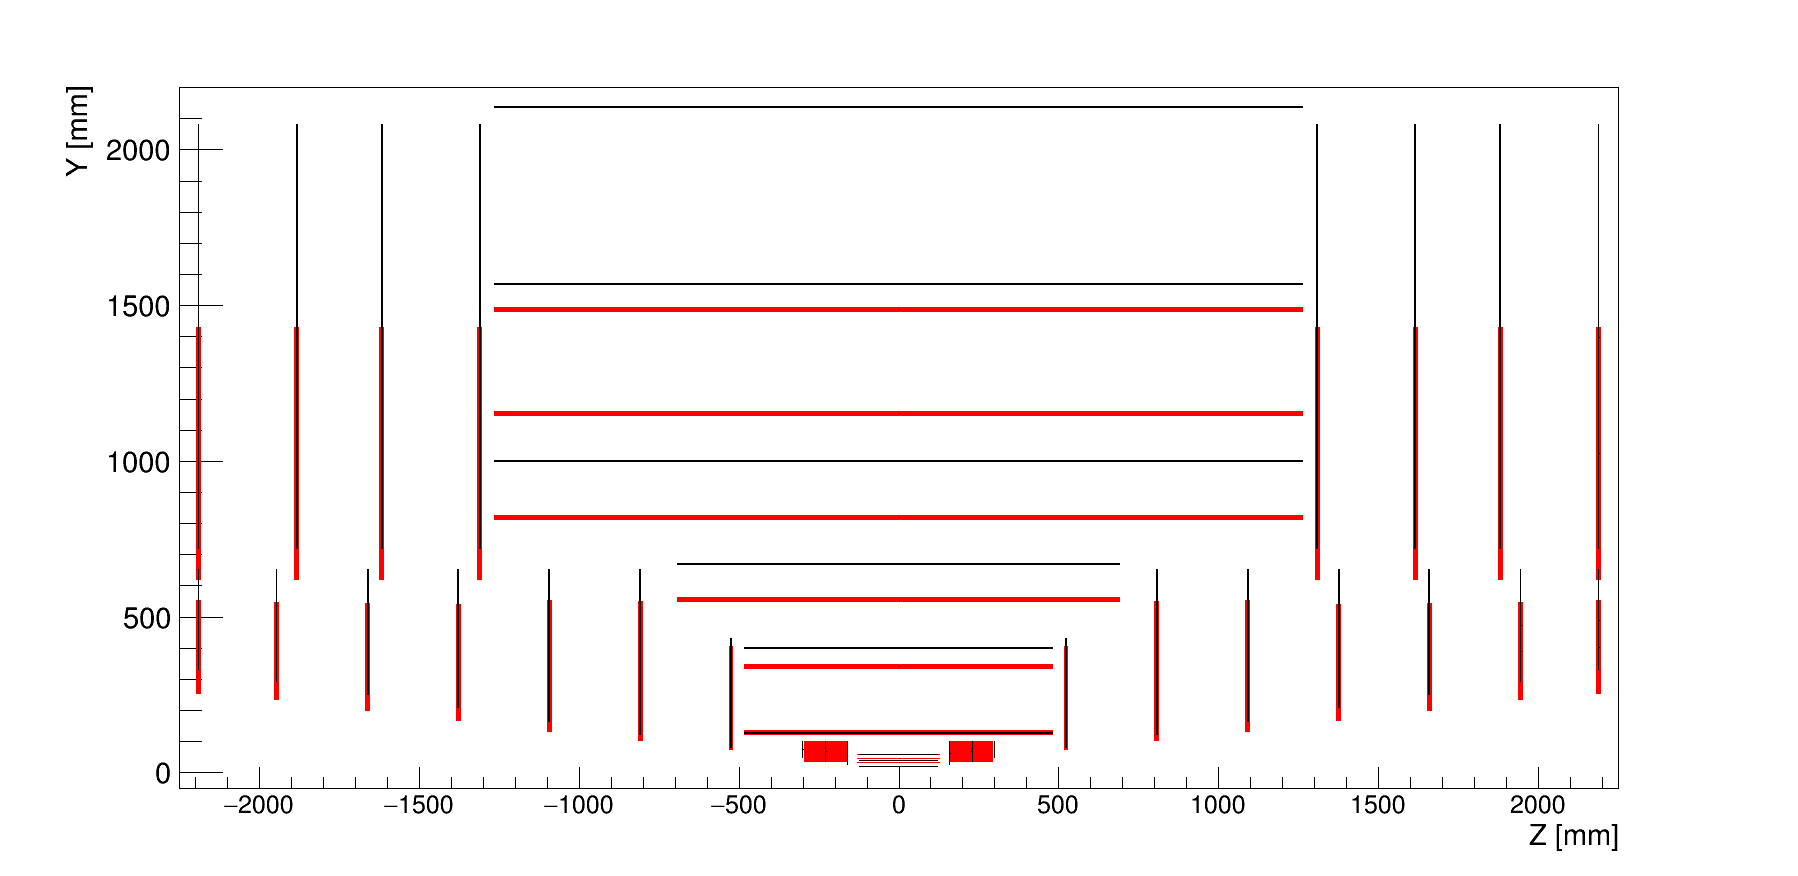
\includegraphics[width=12cm]{CLIC_vs_FCCee_trackingSystem.png}};


 \node[inner sep=0pt] (tmp) at (\xRefPosOne,\yRefPosOne)
%     {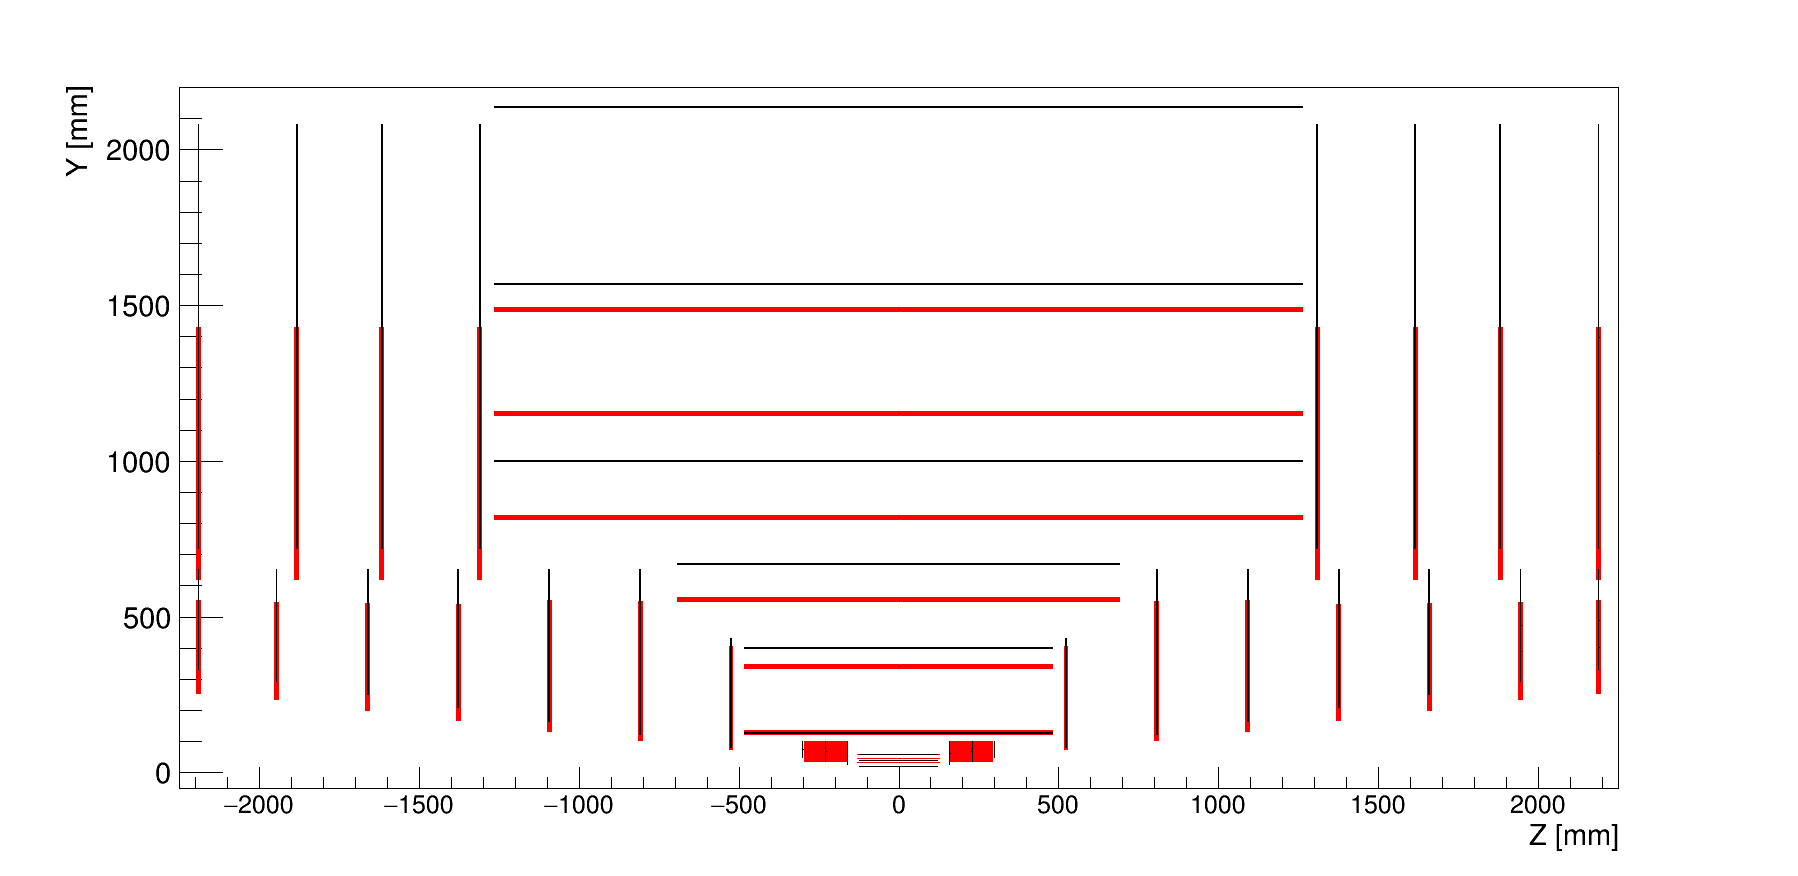
\includegraphics[width=12cm]{CLIC_vs_FCCee_trackingSystem.png}};
  {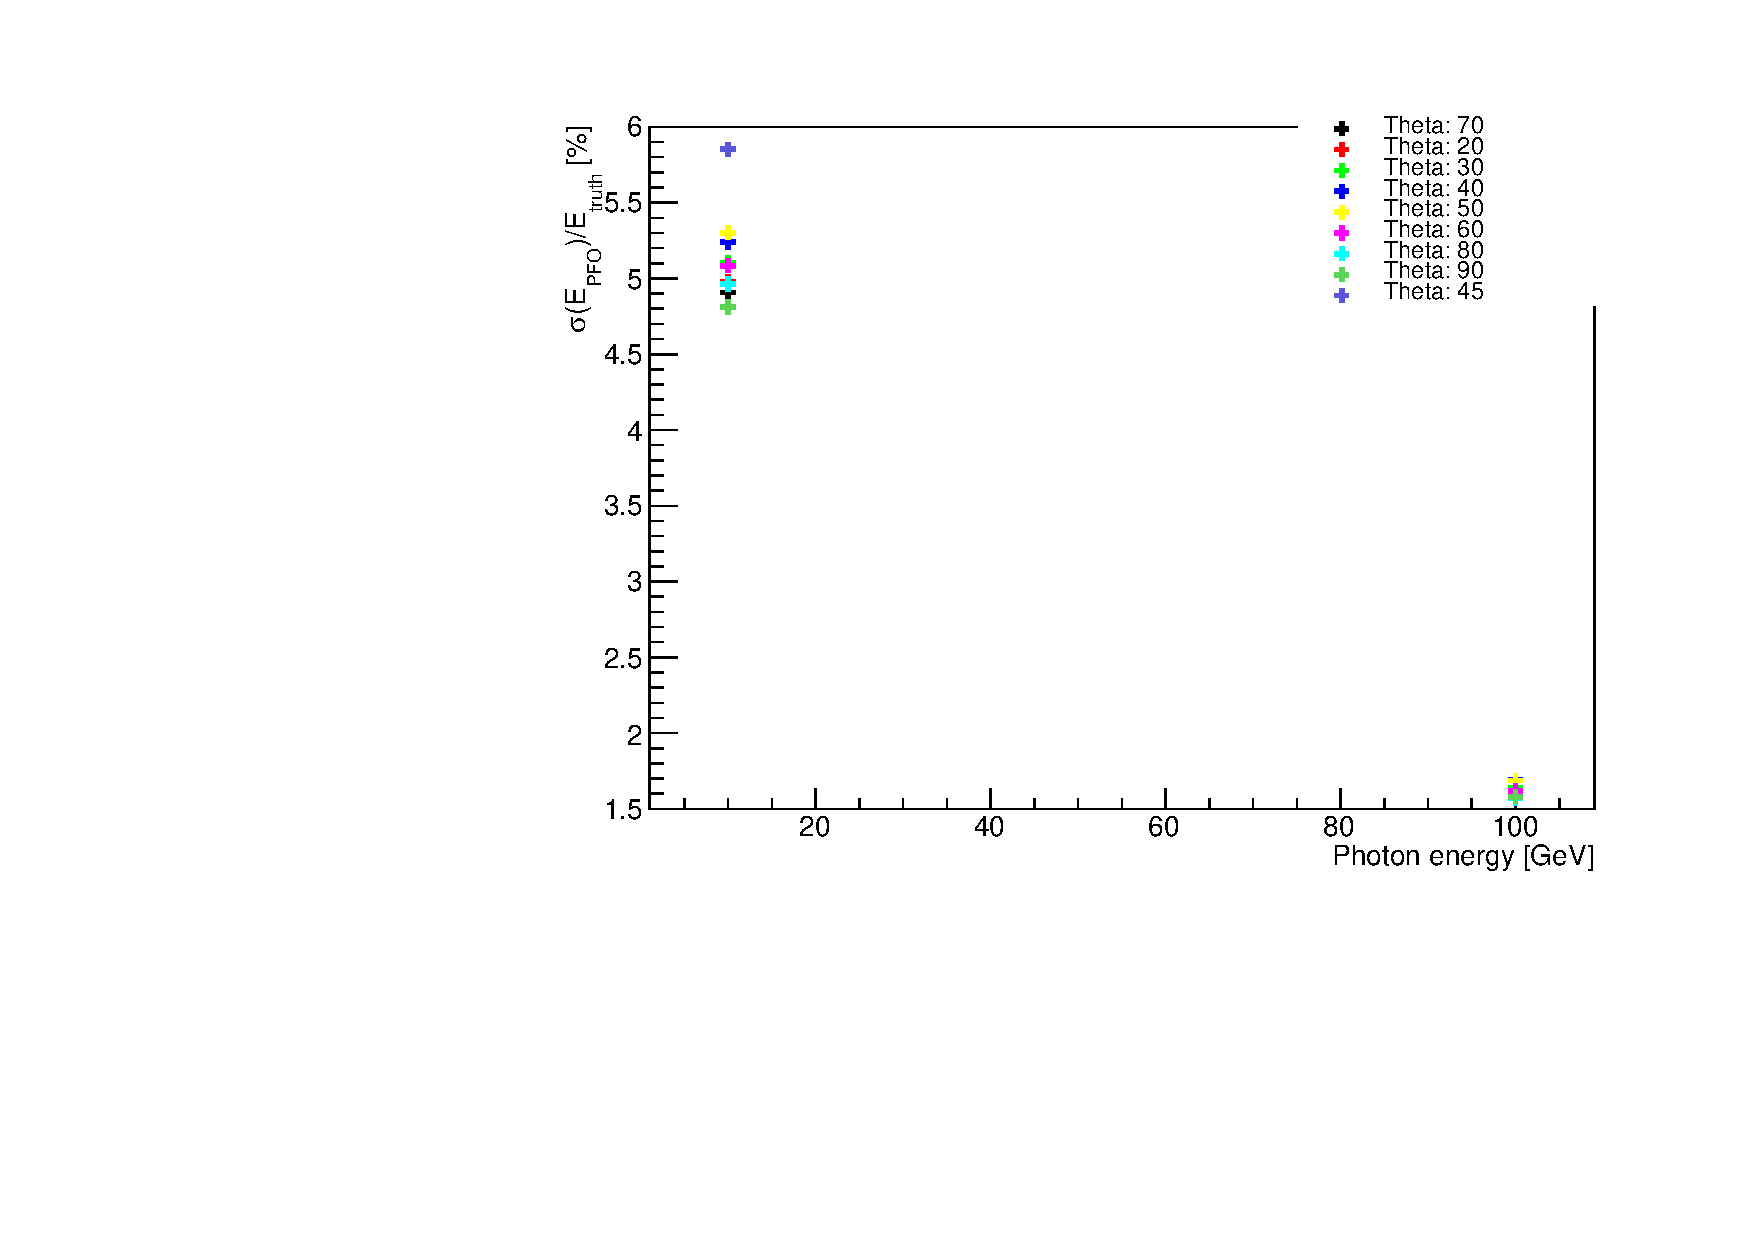
\includegraphics[width=7cm]{energyResolution_energy.pdf}};

 \node[inner sep=0pt] (tmp) at (\xRefPosOne+6,\yRefPosOne)
%     {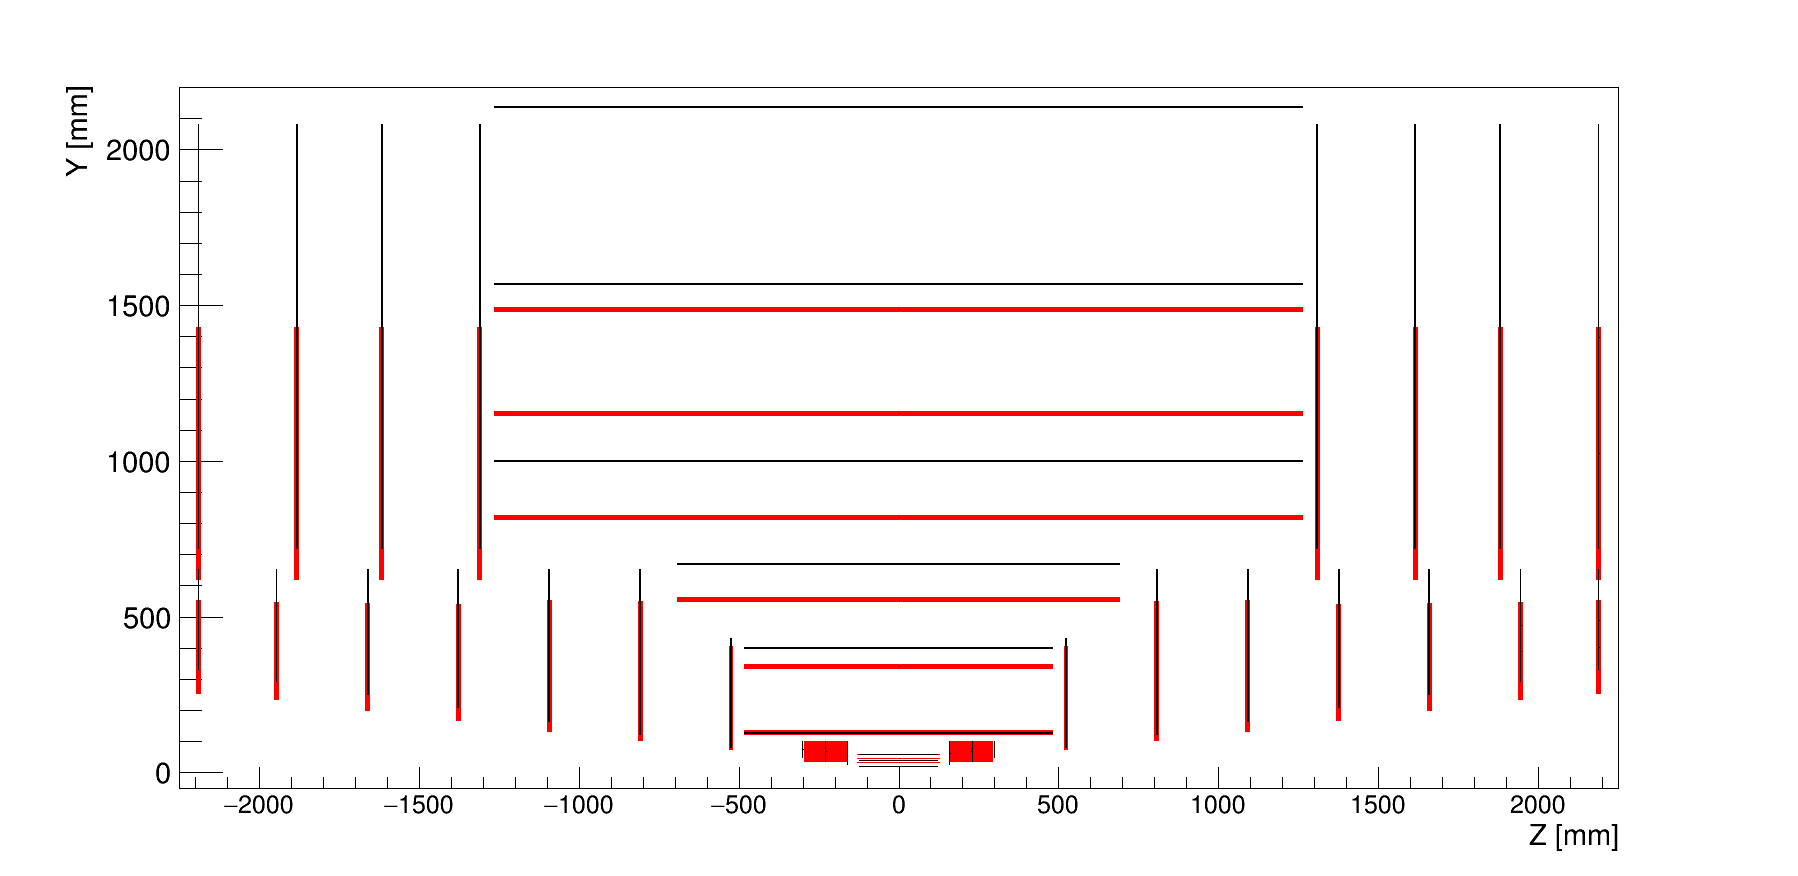
\includegraphics[width=12cm]{CLIC_vs_FCCee_trackingSystem.png}};
  {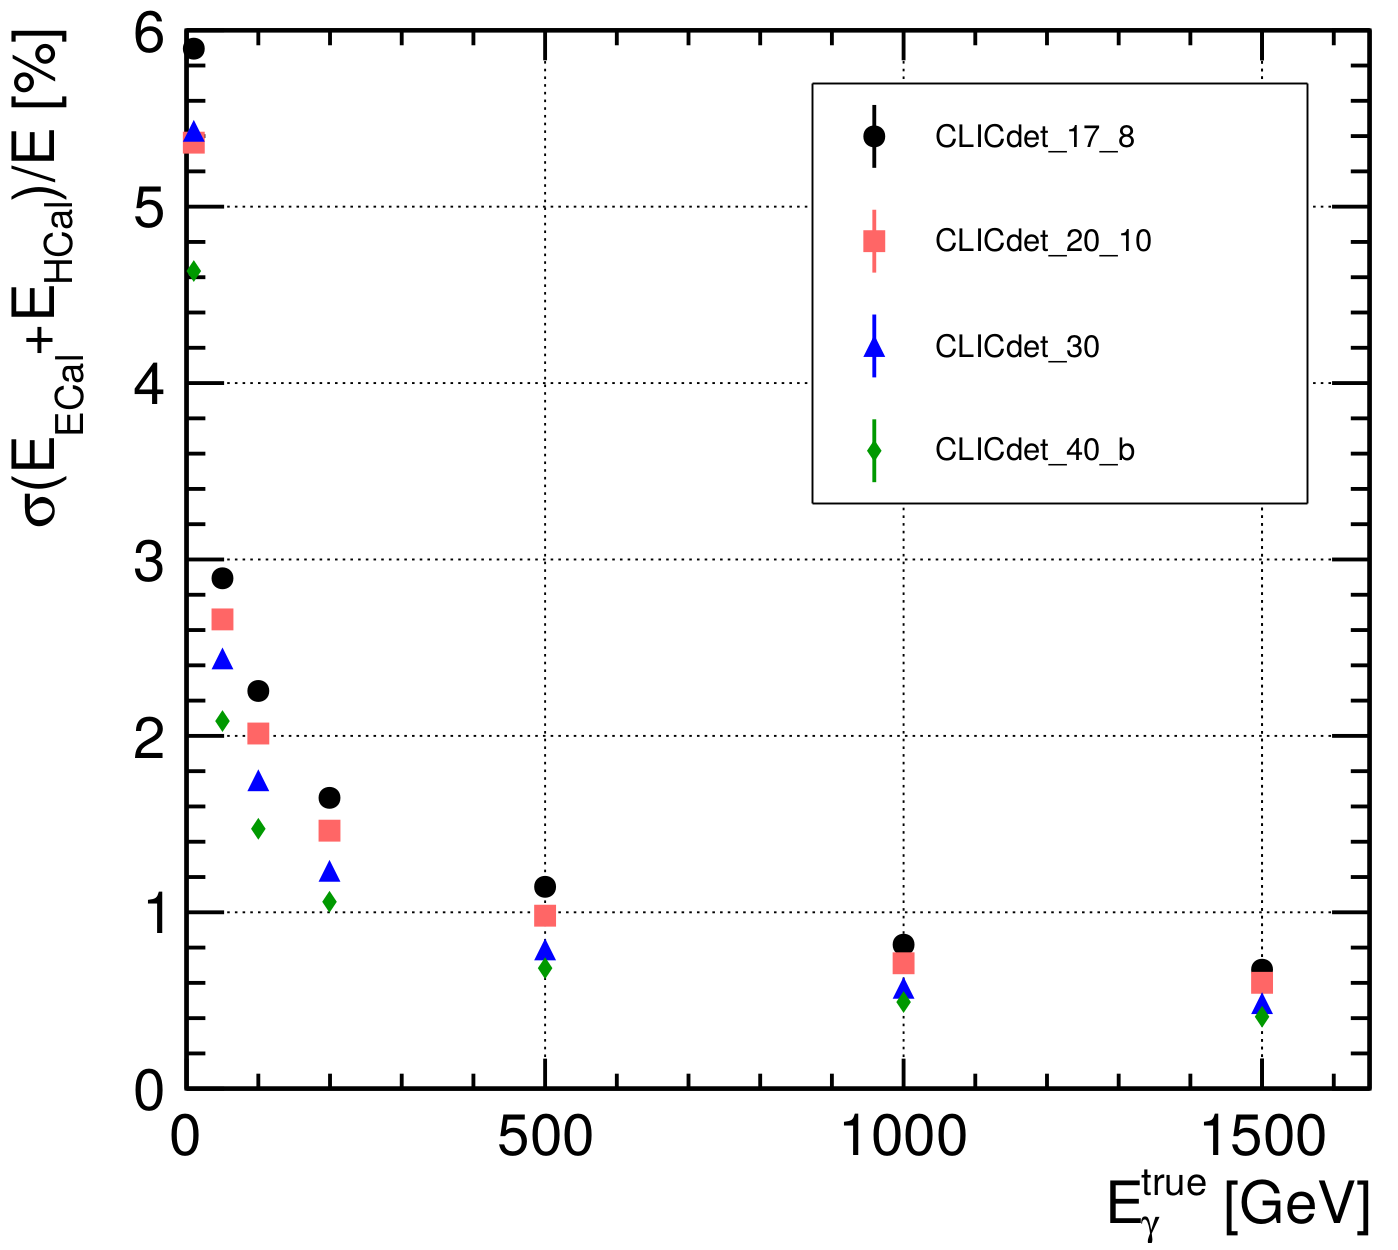
\includegraphics[width=6cm]{../ECAL_res.png}};

% 
\node [Box] at (\xRefPosOne,\yRefPosOne+1.5) (box){%
\myCenterBox{FCCee}
};
% \node [Box] at (\xRefPosOne-2,\yRefPosOne+2) (box){%
% \myCenterBox{theta 80}
% };    
% 
\node [Box] at (\xRefPosOne+5,\yRefPosOne+1.5) (box){%
\myCenterBox{CLIC}
};
\node [Box] at (\xRefPosOne+5,\yRefPosOne+1) (box){%
\myCenterBox{theta 90}
};
% \node [Box] at (\xRefPosOne-2,\yRefPosOne-2.1) (box){%
% \myCenterBox{theta 80}
% };    
% 
\node [Box] at (\xRefPosOne+1,\yRefPosOne-3) (box){%
  \begin{minipage}{0.7\textwidth}
    \begin{itemize}
      \item Energy resolution is similar to the CLIC one
    \end{itemize}
  \end{minipage}
};
%     
%% HELPER draw advanced helping grid with axises:
% \draw(-0.5,-4) to[grid with coordinates] (11.5,4);
\end{tikzpicture}

  
\end{frame}
%*****************************************************************************


%*****************************************************************************
\begin{frame}{\large \large Reconstructed energy}
 
\renewcommand{\yRefPosOne}{0}
\renewcommand{\xRefPosOne}{2.5}
\renewcommand{\xRefIncrementOne}{5.5}
\begin{tikzpicture}[overlay]

%  \node[inner sep=0pt] (tmp) at (\xRefPosOne,\yRefPosOne-1.9)
%     {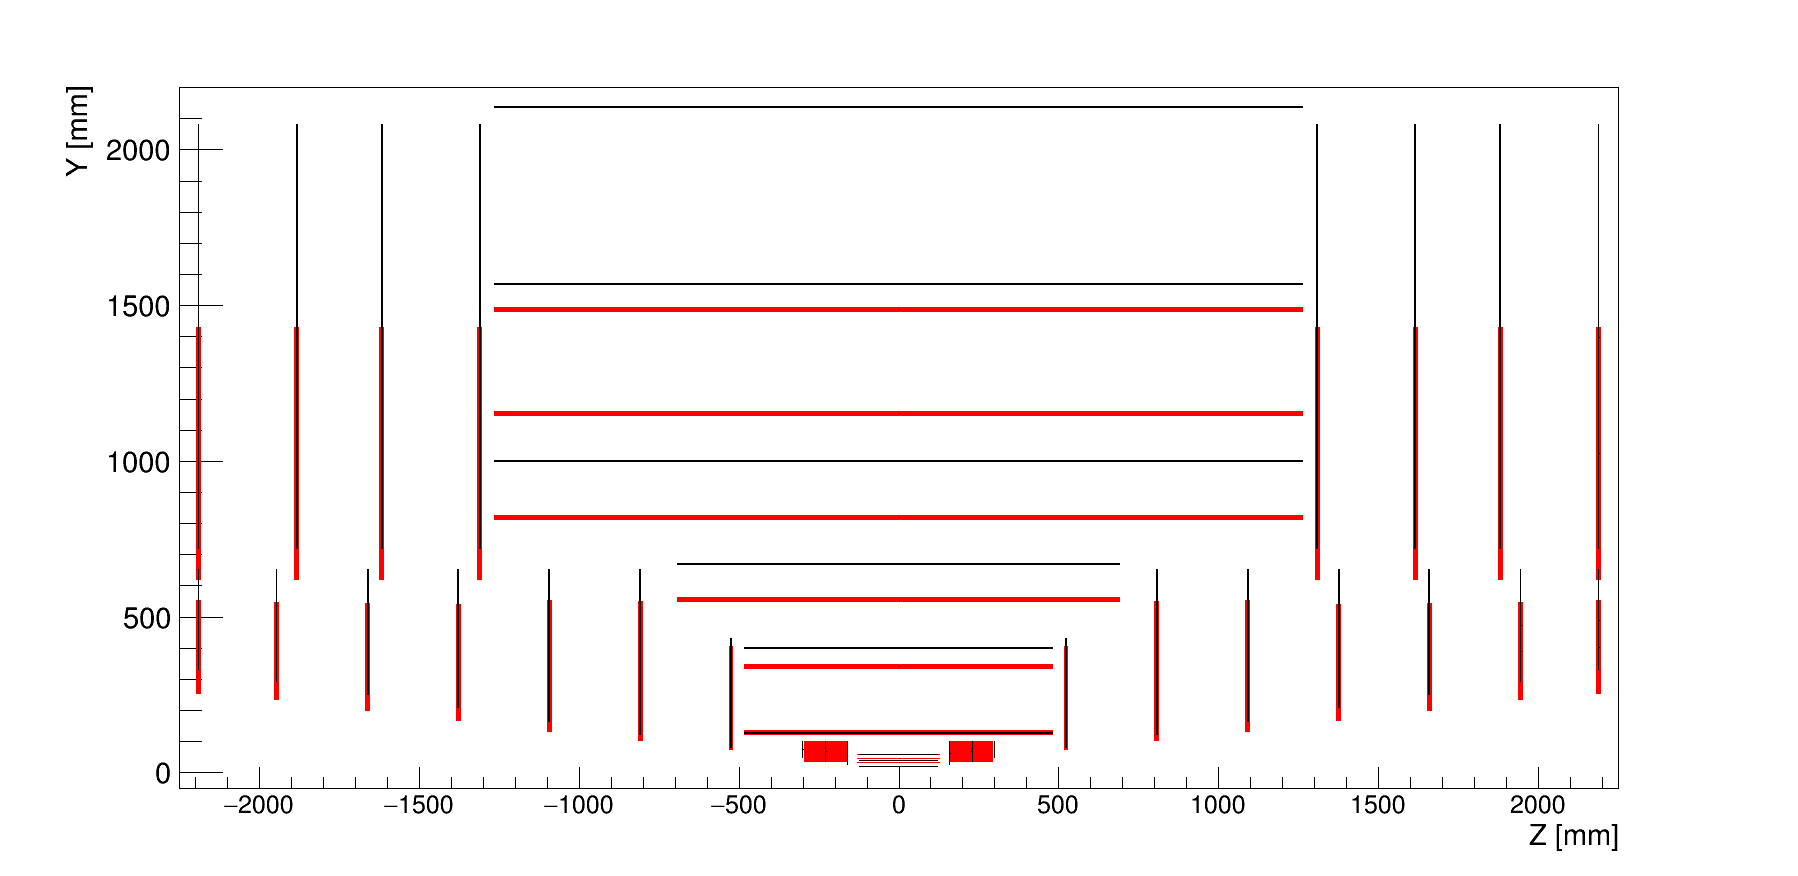
\includegraphics[width=12cm]{CLIC_vs_FCCee_trackingSystem.png}};


 \node[inner sep=0pt] (tmp) at (\xRefPosOne,\yRefPosOne+1.2)
%     {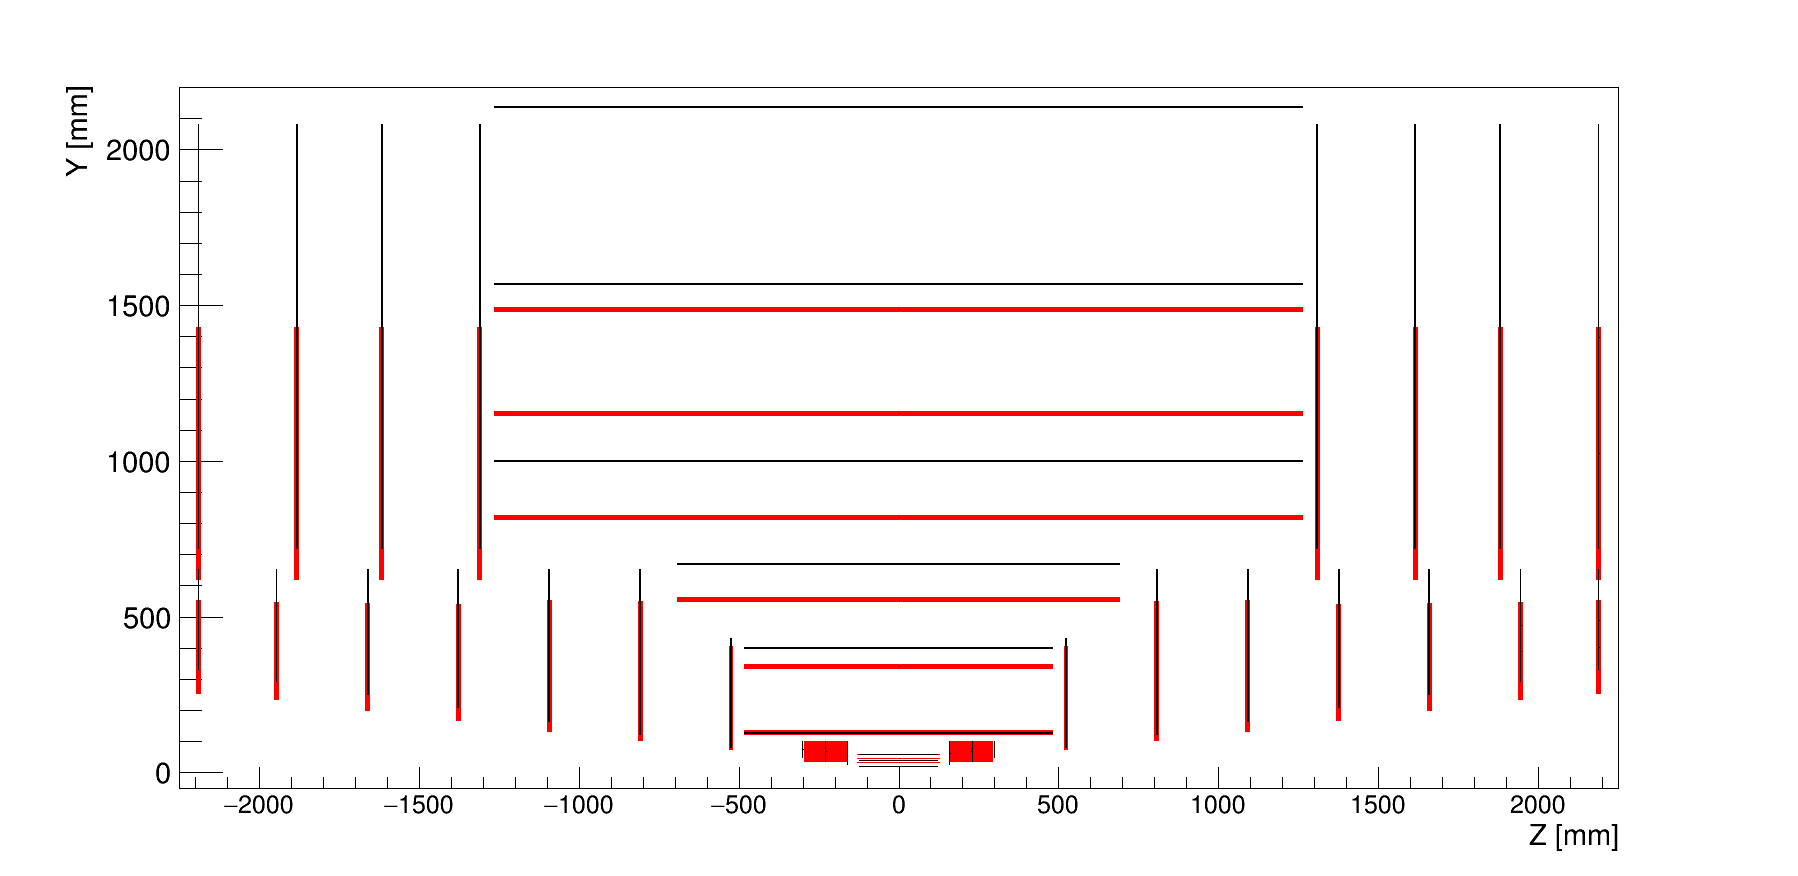
\includegraphics[width=12cm]{CLIC_vs_FCCee_trackingSystem.png}};
  {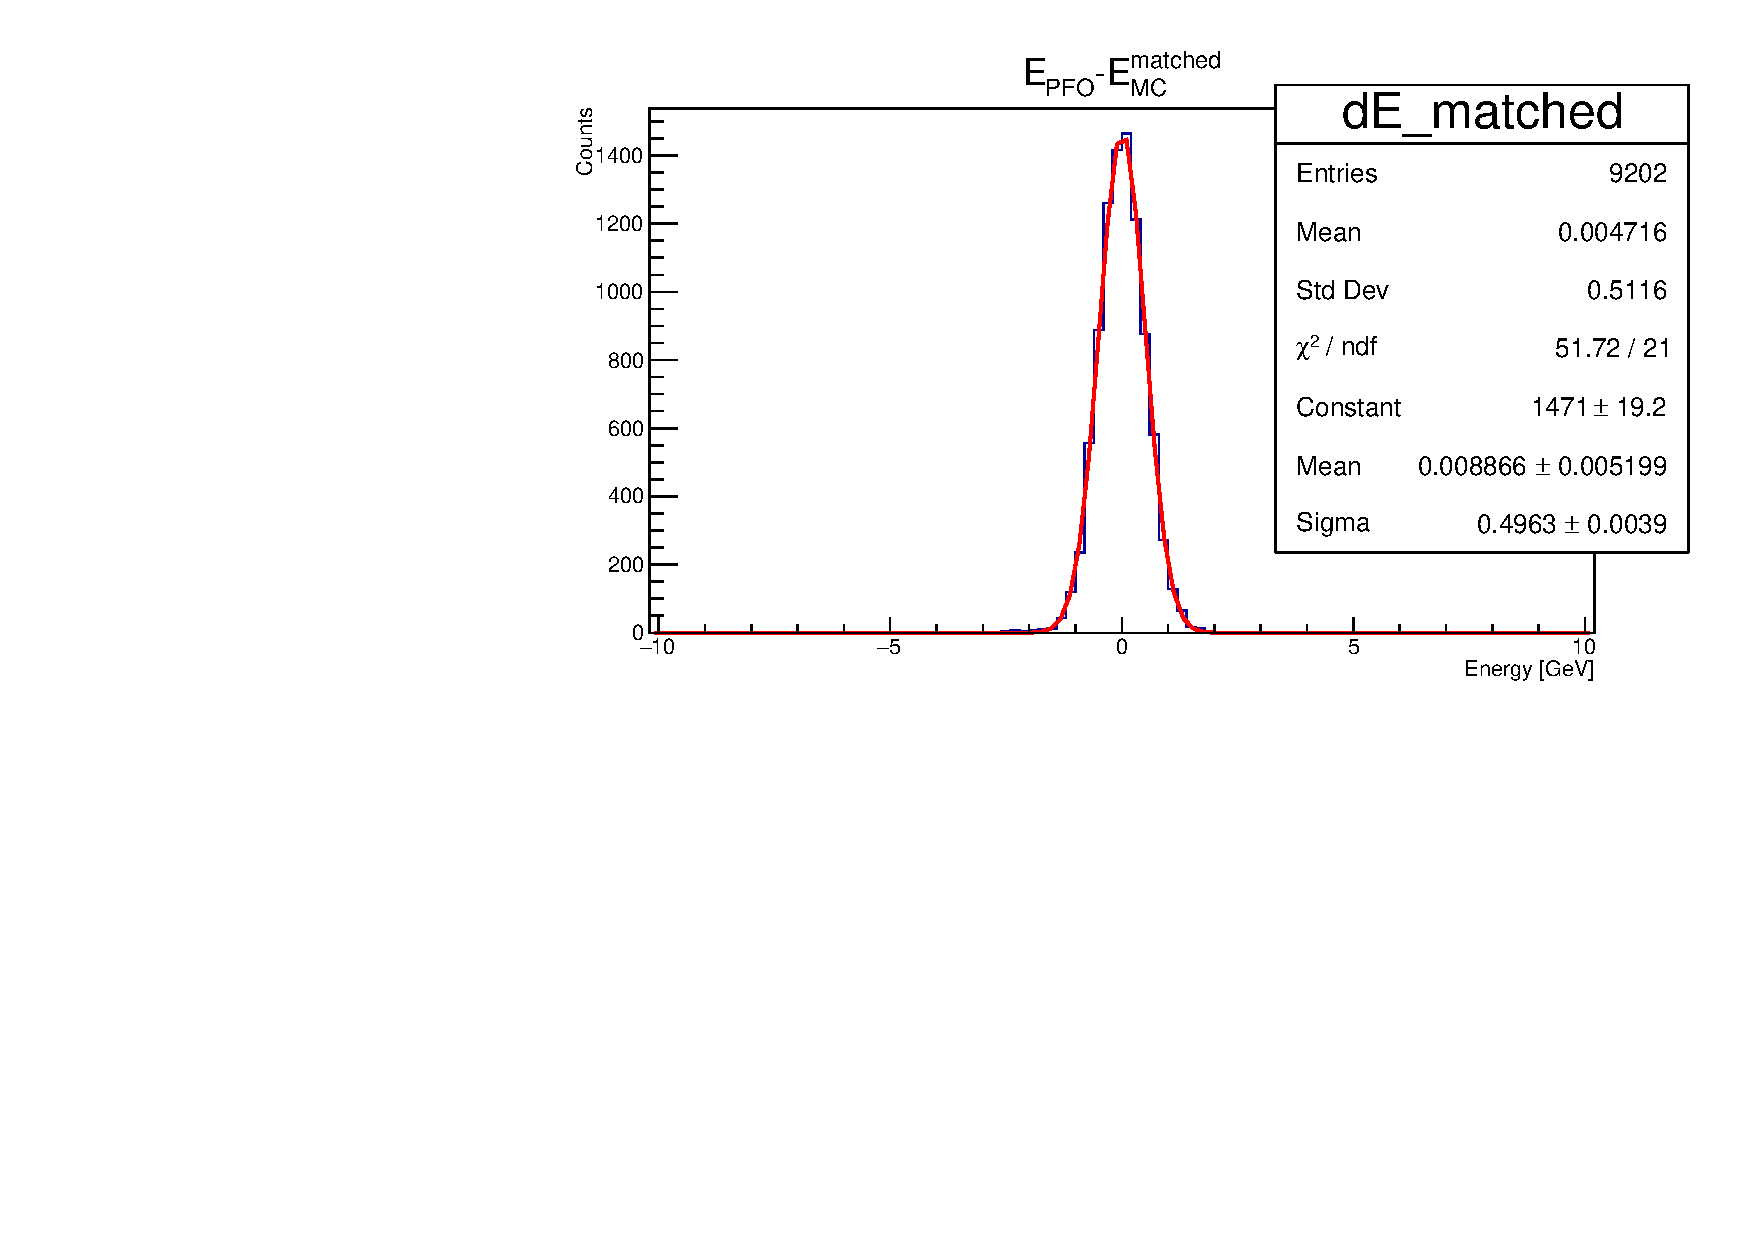
\includegraphics[width=7cm]{dEFit_E10_theta80.pdf}};

 \node[inner sep=0pt] (tmp) at (\xRefPosOne,\yRefPosOne-2.9)
%     {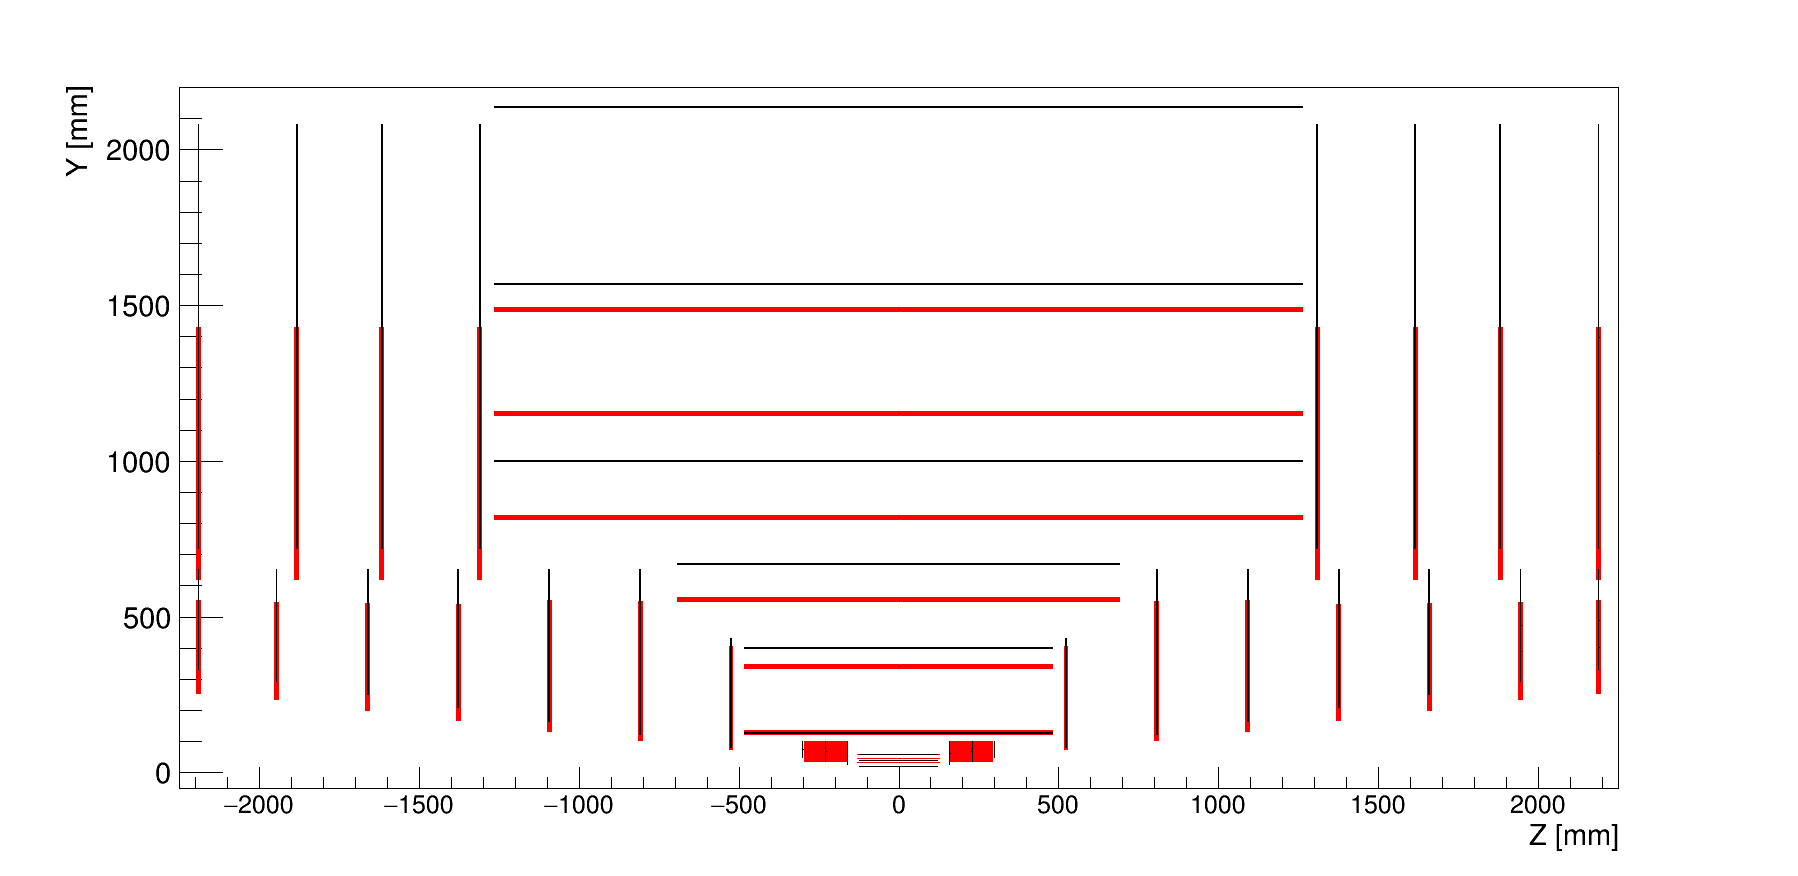
\includegraphics[width=12cm]{CLIC_vs_FCCee_trackingSystem.png}};
  {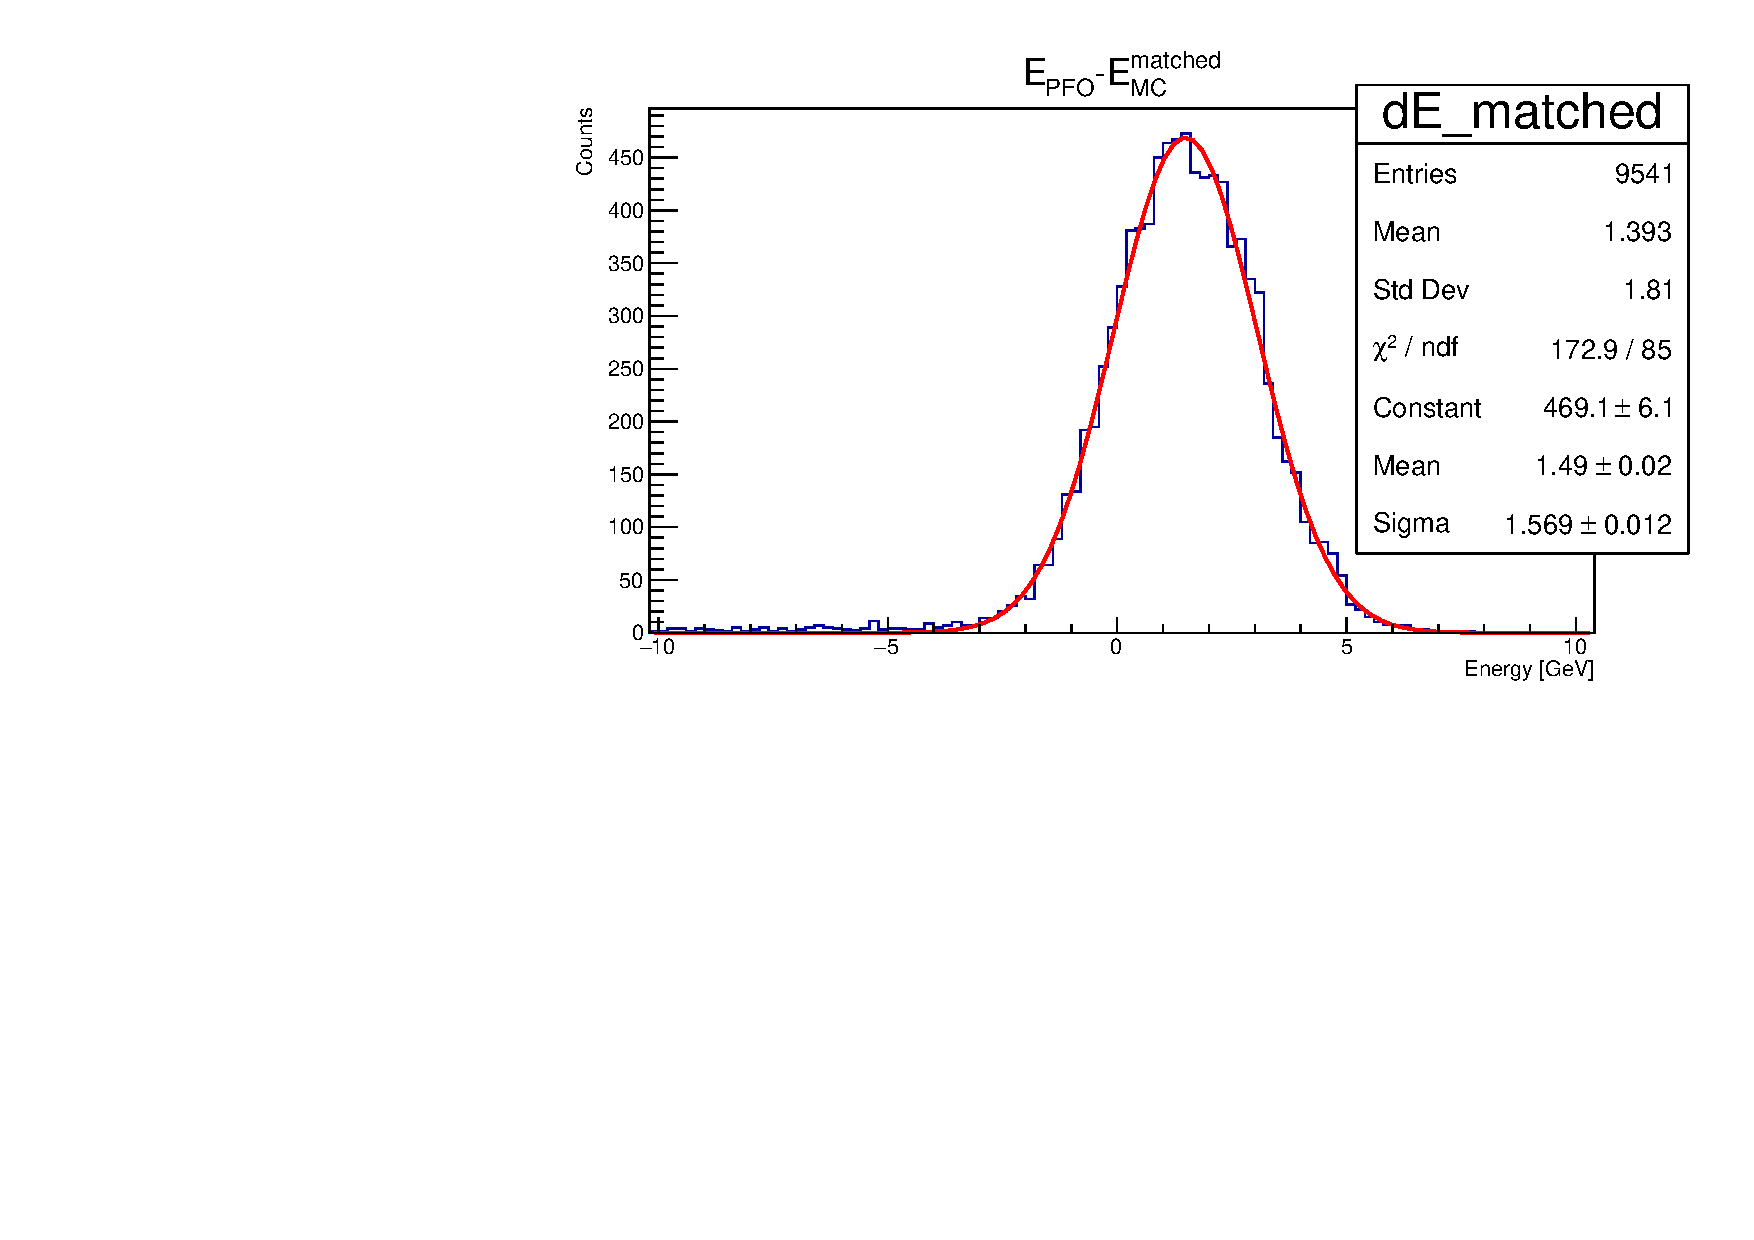
\includegraphics[width=7cm]{dEFit_E100_theta80.pdf}};


\node [Box] at (\xRefPosOne-2,\yRefPosOne+2.4) (box){%
\myCenterBox{10 GeV}
};
\node [Box] at (\xRefPosOne-2,\yRefPosOne+2) (box){%
\myCenterBox{theta 80}
};    

\node [Box] at (\xRefPosOne-2,\yRefPosOne-1.7) (box){%
\myCenterBox{100 GeV}
};
\node [Box] at (\xRefPosOne-2,\yRefPosOne-2.1) (box){%
\myCenterBox{theta 80}
};    

\node [Box] at (\xRefPosOne+6,\yRefPosOne) (box){%
  \begin{minipage}{0.5\textwidth}
    \begin{itemize}
      \item Bias of the reconstructed energy wrt to truth photon energy \\ \vspace{1cm}
      \item Effect is also observed for CLIC detector (1.8$\%$ at 100 GeV)
    \end{itemize}
  \end{minipage}
};
    
%% HELPER draw advanced helping grid with axises:
% \draw(-0.5,-4) to[grid with coordinates] (11.5,4);
\end{tikzpicture}

  
\end{frame}
%*****************************************************************************

%*****************************************************************************
\begin{frame}{\large \large Photon Energy Scale Bias}
 
\renewcommand{\yRefPosOne}{0}
\renewcommand{\xRefPosOne}{2.5}
\renewcommand{\xRefIncrementOne}{5.5}
\begin{tikzpicture}[overlay]

%  \node[inner sep=0pt] (tmp) at (\xRefPosOne,\yRefPosOne-1.9)
%     {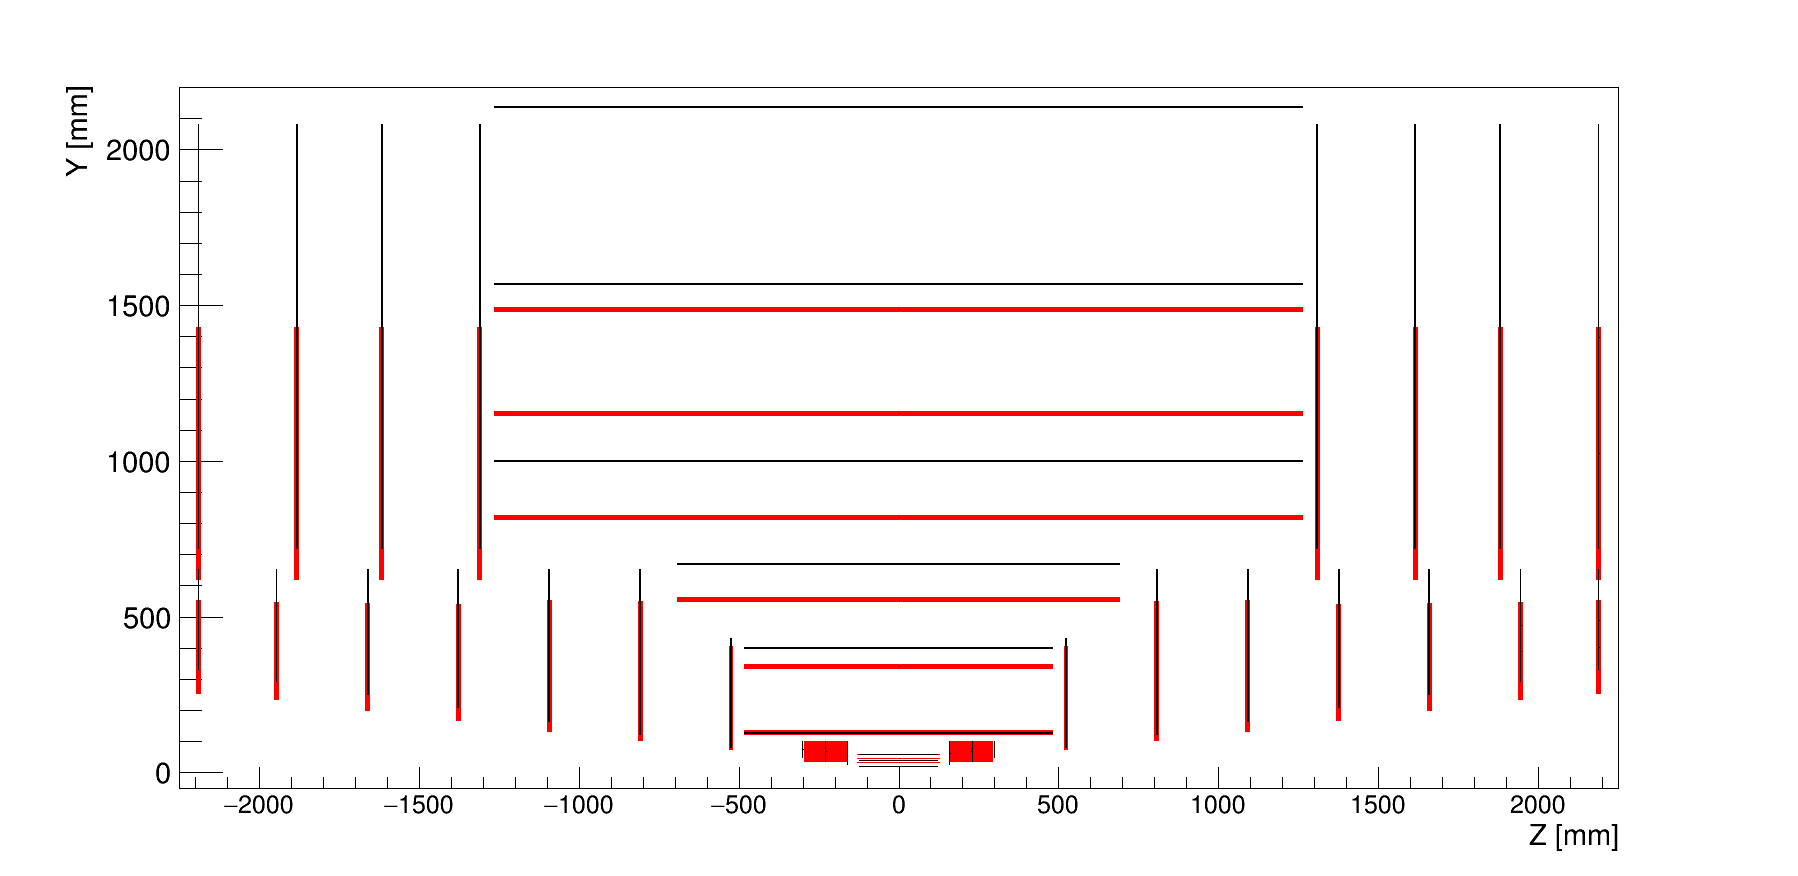
\includegraphics[width=12cm]{CLIC_vs_FCCee_trackingSystem.png}};


 \node[inner sep=0pt] (tmp) at (\xRefPosOne,\yRefPosOne)
%     {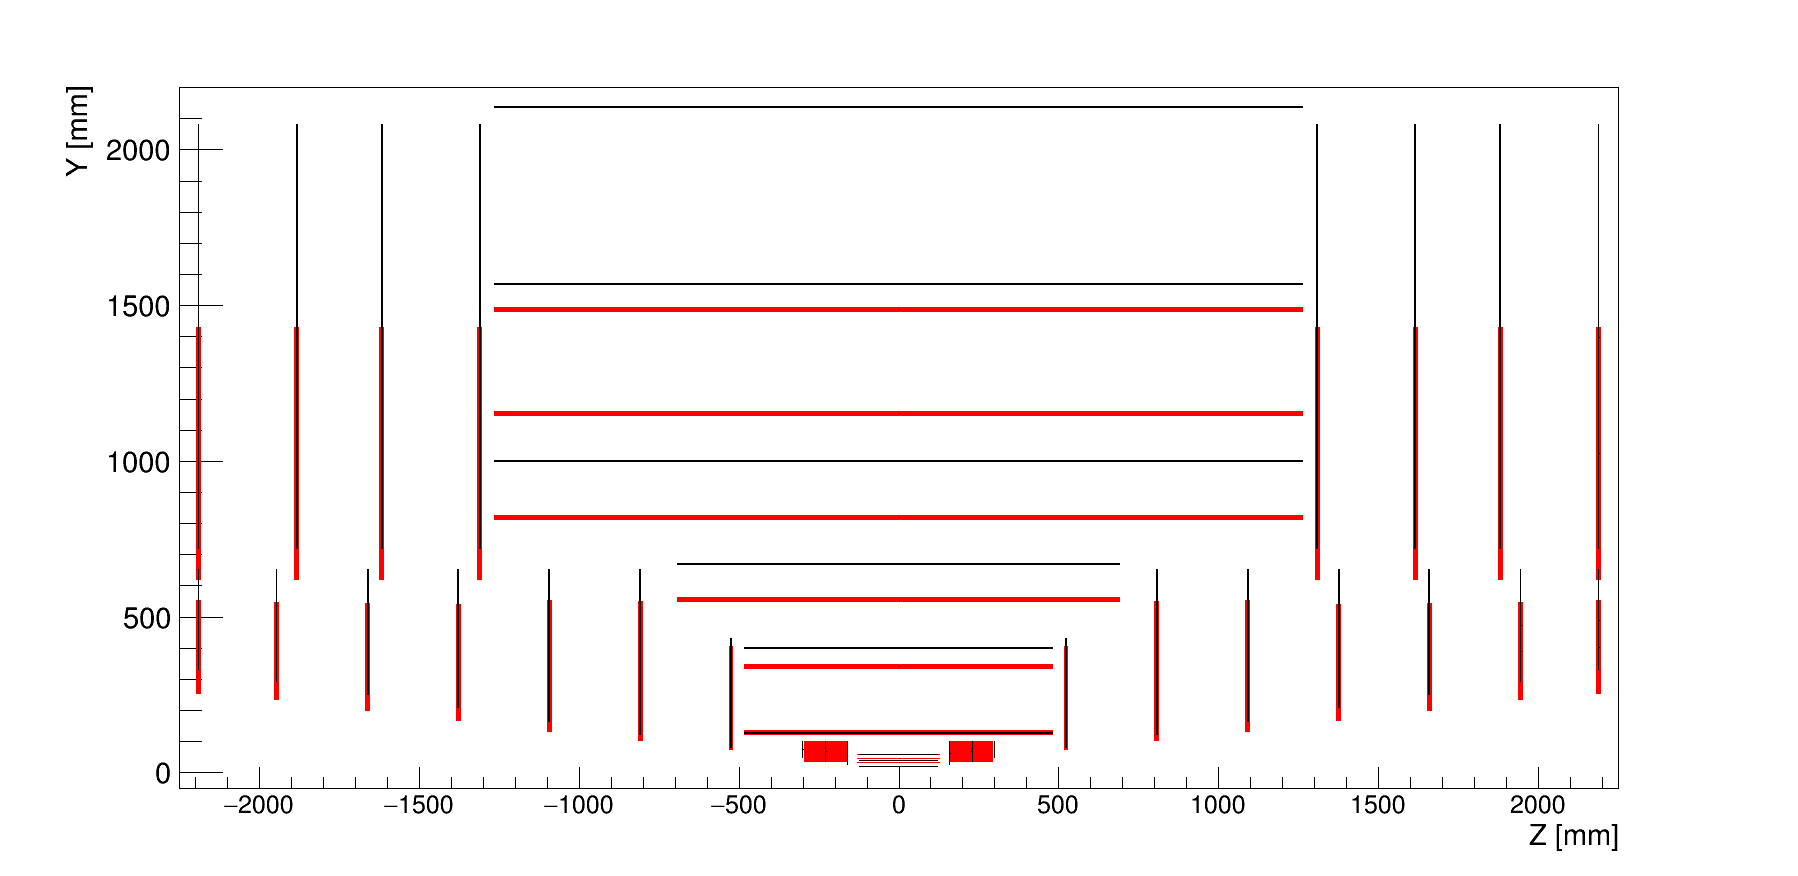
\includegraphics[width=12cm]{CLIC_vs_FCCee_trackingSystem.png}};
  {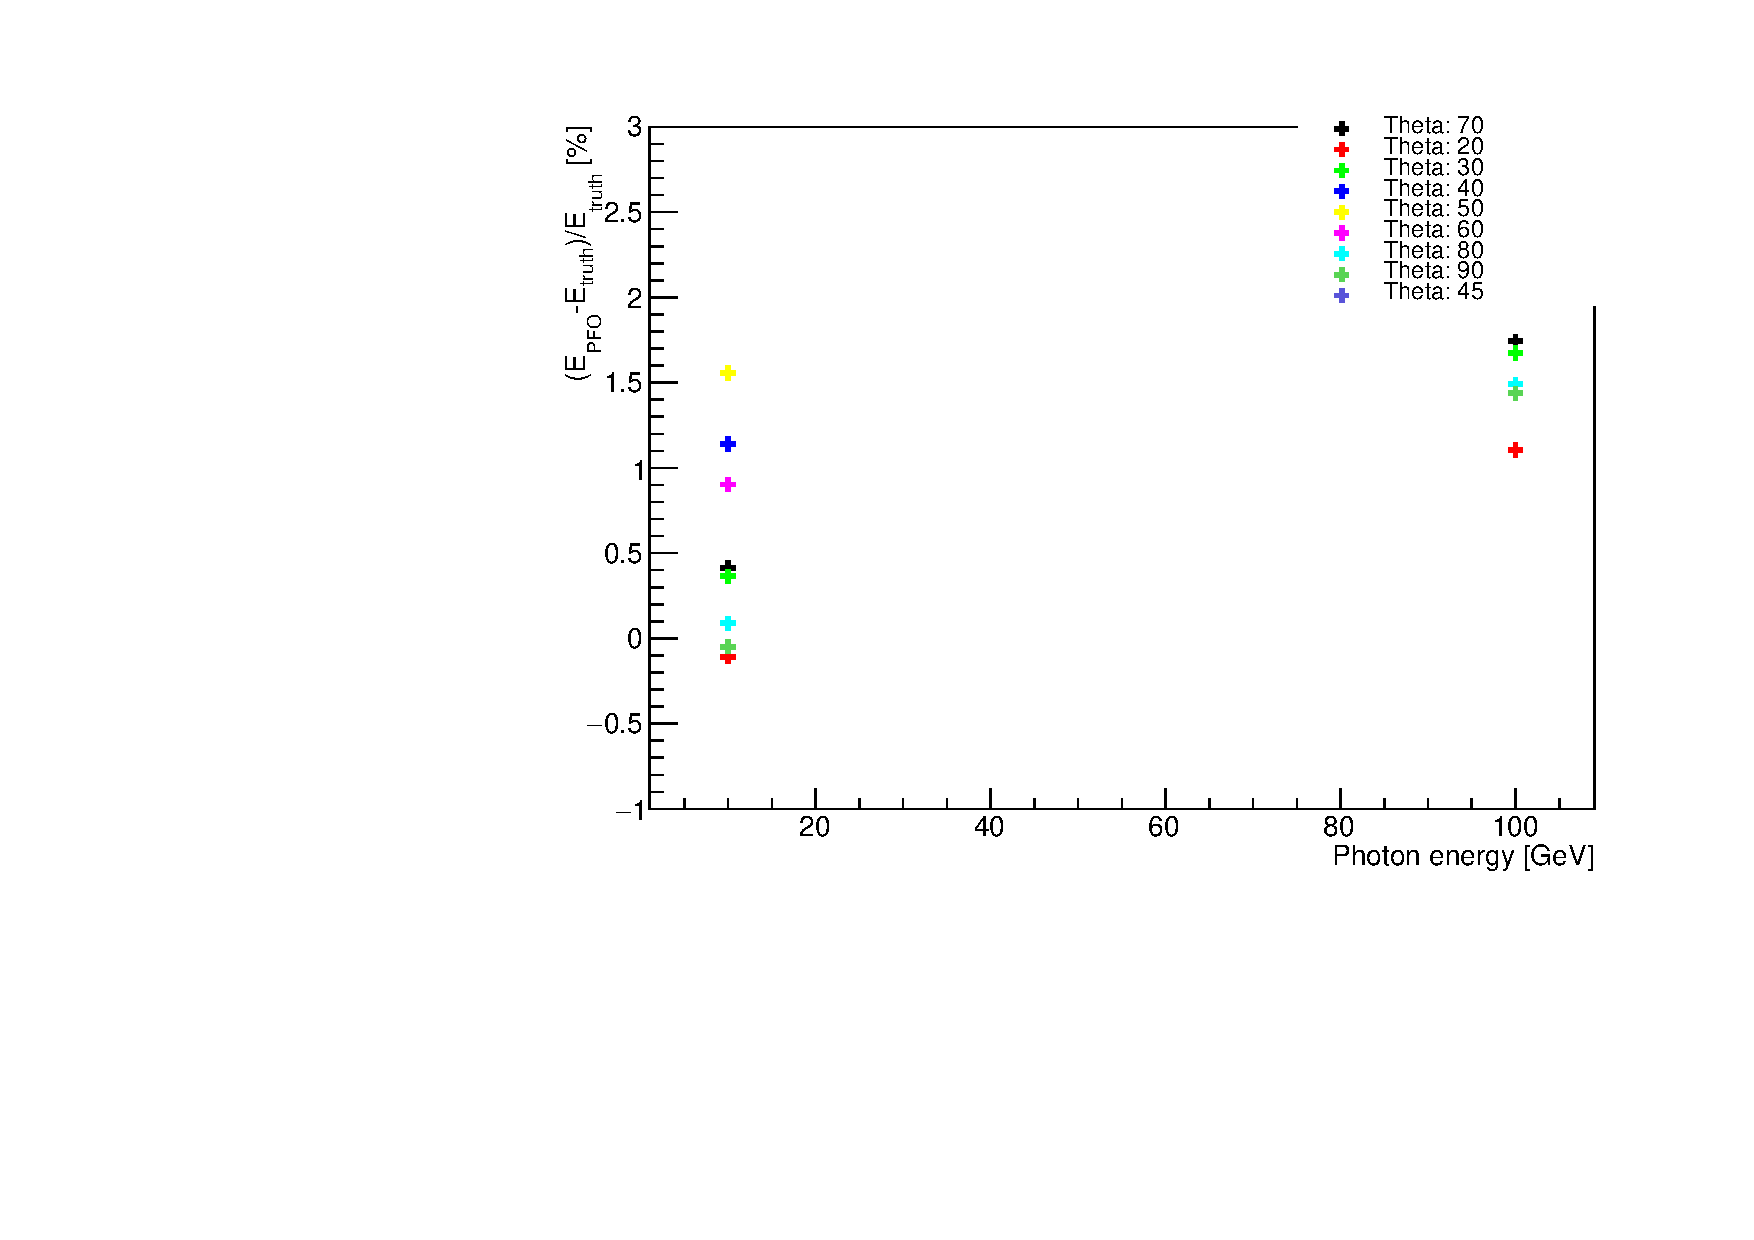
\includegraphics[width=6.5cm]{energyScaleBias_energy.pdf}};

 \node[inner sep=0pt] (tmp) at (\xRefPosOne+6,\yRefPosOne)
%     {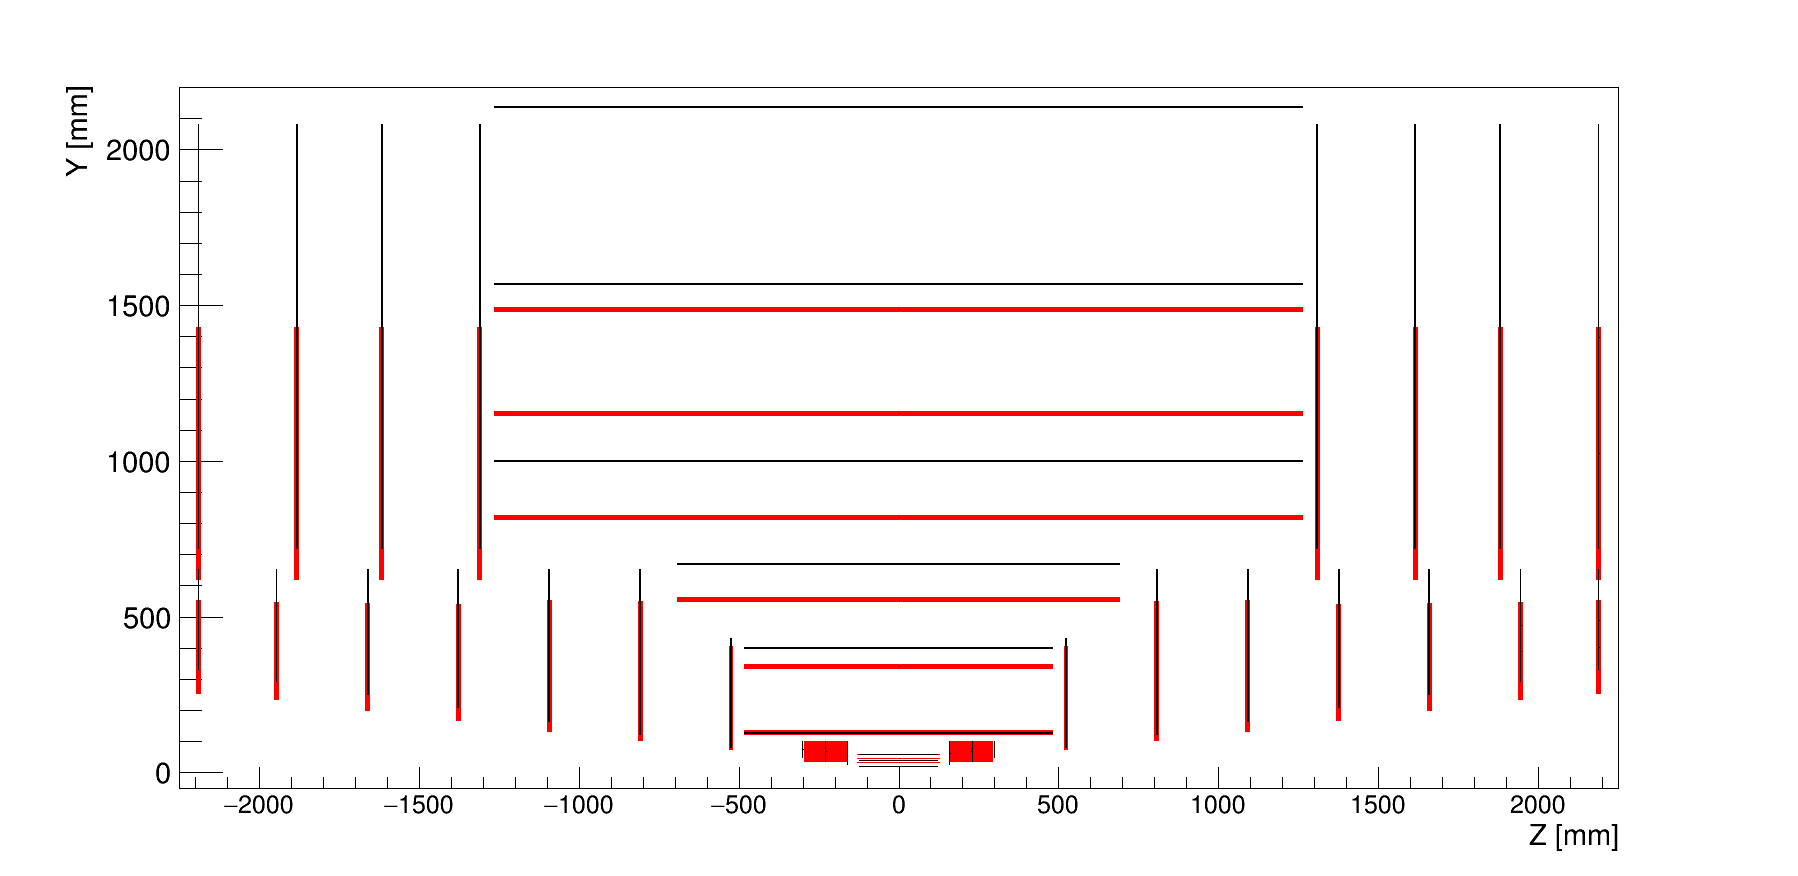
\includegraphics[width=12cm]{CLIC_vs_FCCee_trackingSystem.png}};
  {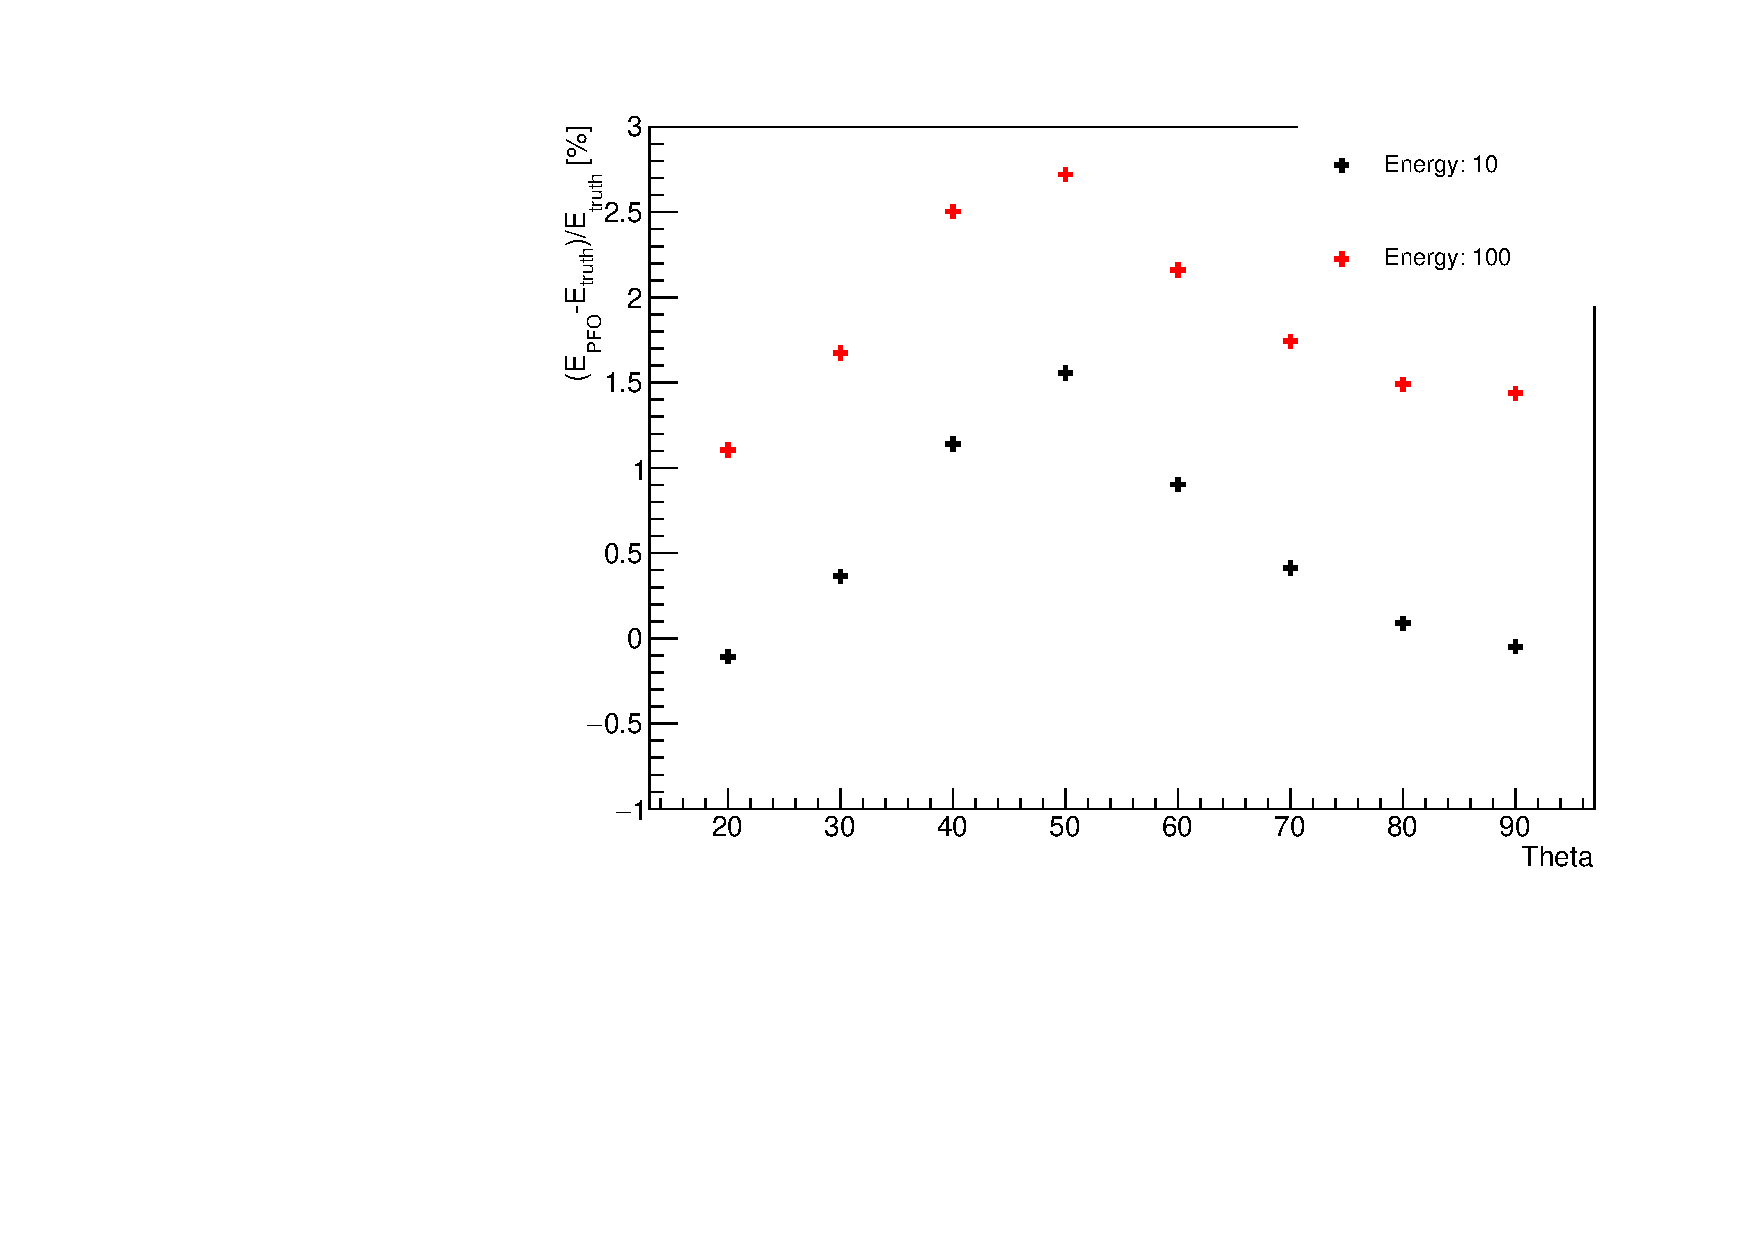
\includegraphics[width=6.5cm]{energyScaleBias_theta.pdf}};

% 
% \node [Box] at (\xRefPosOne,\yRefPosOne+1.5) (box){%
% \myCenterBox{FCCee}
% };
% \node [Box] at (\xRefPosOne-2,\yRefPosOne+2) (box){%
% \myCenterBox{theta 80}
% };    
% 
% \node [Box] at (\xRefPosOne+5,\yRefPosOne+1.5) (box){%
% \myCenterBox{CLIC}
% };
% \node [Box] at (\xRefPosOne+5,\yRefPosOne+1) (box){%
% \myCenterBox{theta 90}
% };
% \node [Box] at (\xRefPosOne-2,\yRefPosOne-2.1) (box){%
% \myCenterBox{theta 80}
% };    
% 
\node [Box] at (\xRefPosOne+2.5,\yRefPosOne-3) (box){%
  \begin{minipage}{\textwidth}
    \begin{itemize}
      \item Bias in the reconstructed energy depends both from energy and direction ($\theta$)
      \item Need further investigation
    \end{itemize}
  \end{minipage}
};
%     
%% HELPER draw advanced helping grid with axises:
% \draw(-0.5,-4) to[grid with coordinates] (11.5,4);
\end{tikzpicture}

  
\end{frame}
%*****************************************************************************

%*****************************************************************************
\begin{frame}{\large \large Photon Energy Scale Bias}
 
\renewcommand{\yRefPosOne}{0}
\renewcommand{\xRefPosOne}{2.5}
\renewcommand{\xRefIncrementOne}{5.5}
\begin{tikzpicture}[overlay]

%  \node[inner sep=0pt] (tmp) at (\xRefPosOne,\yRefPosOne-1.9)
%     {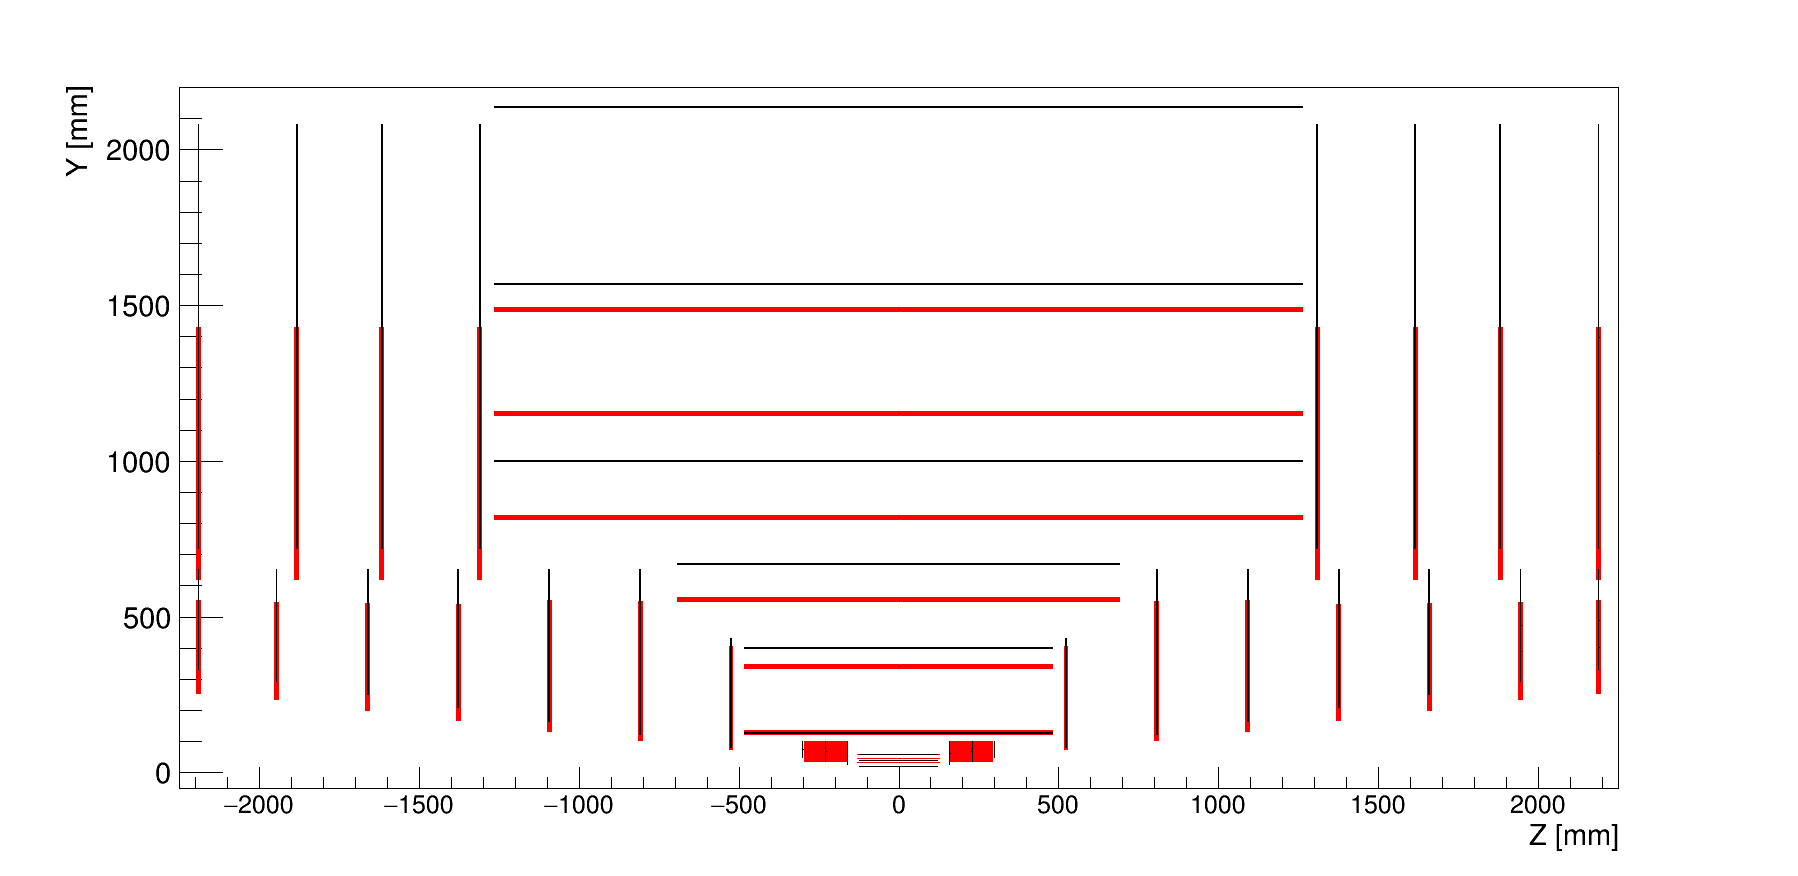
\includegraphics[width=12cm]{CLIC_vs_FCCee_trackingSystem.png}};


 \node[inner sep=0pt] (tmp) at (\xRefPosOne,\yRefPosOne)
%     {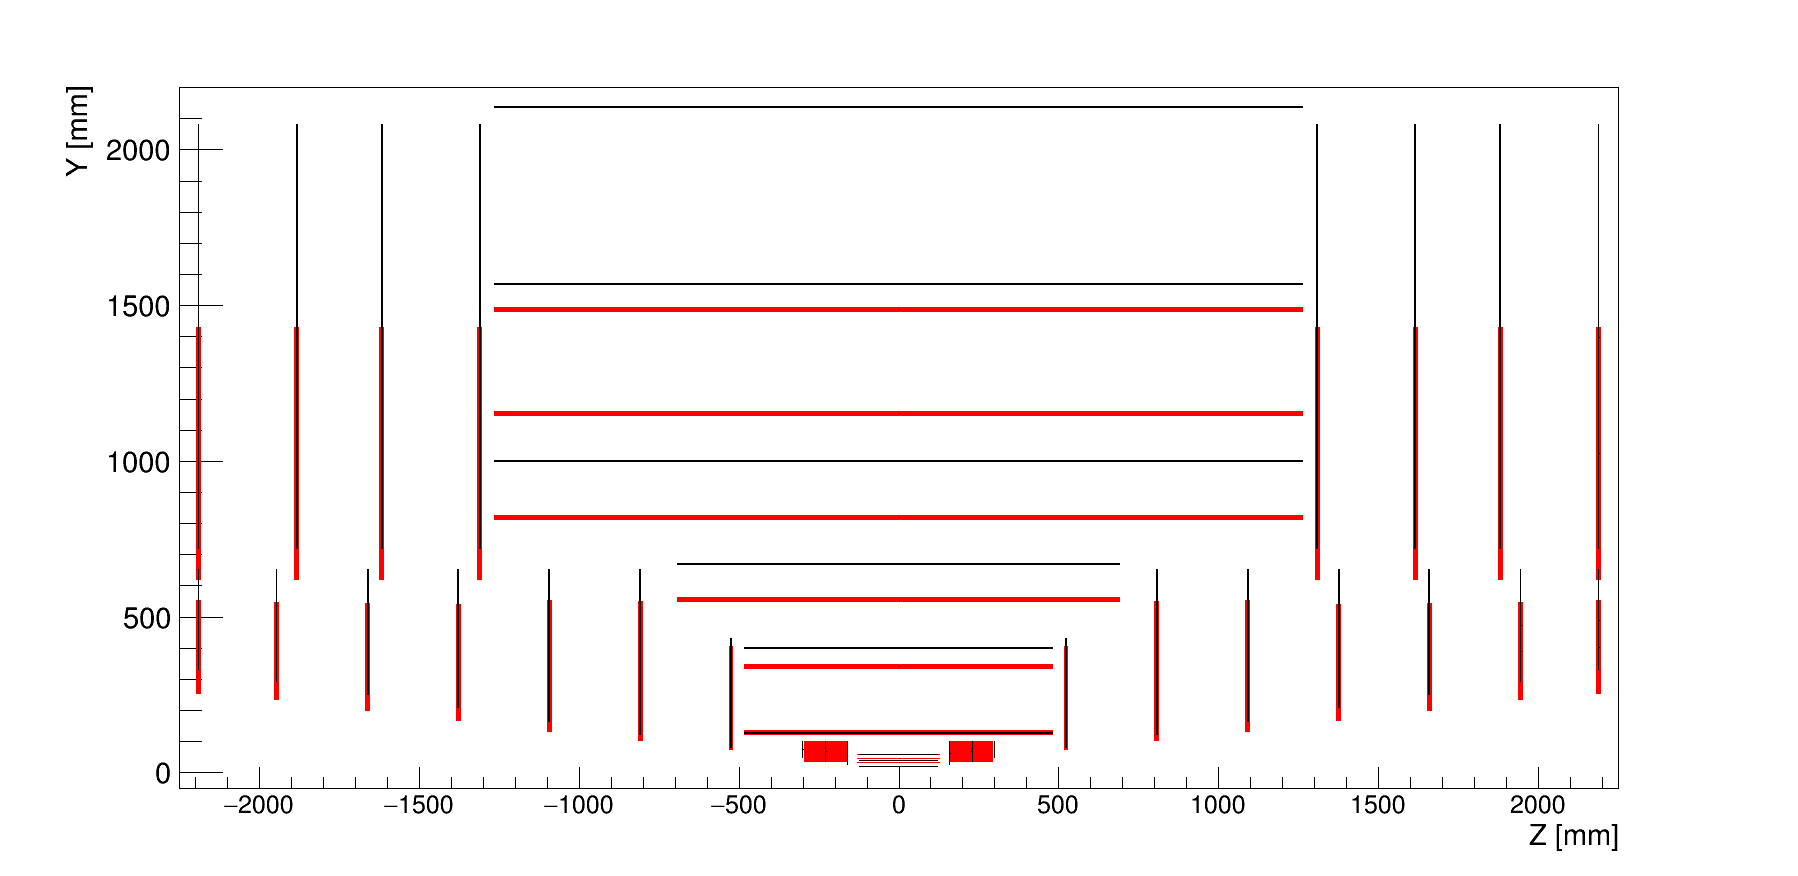
\includegraphics[width=12cm]{CLIC_vs_FCCee_trackingSystem.png}};
  {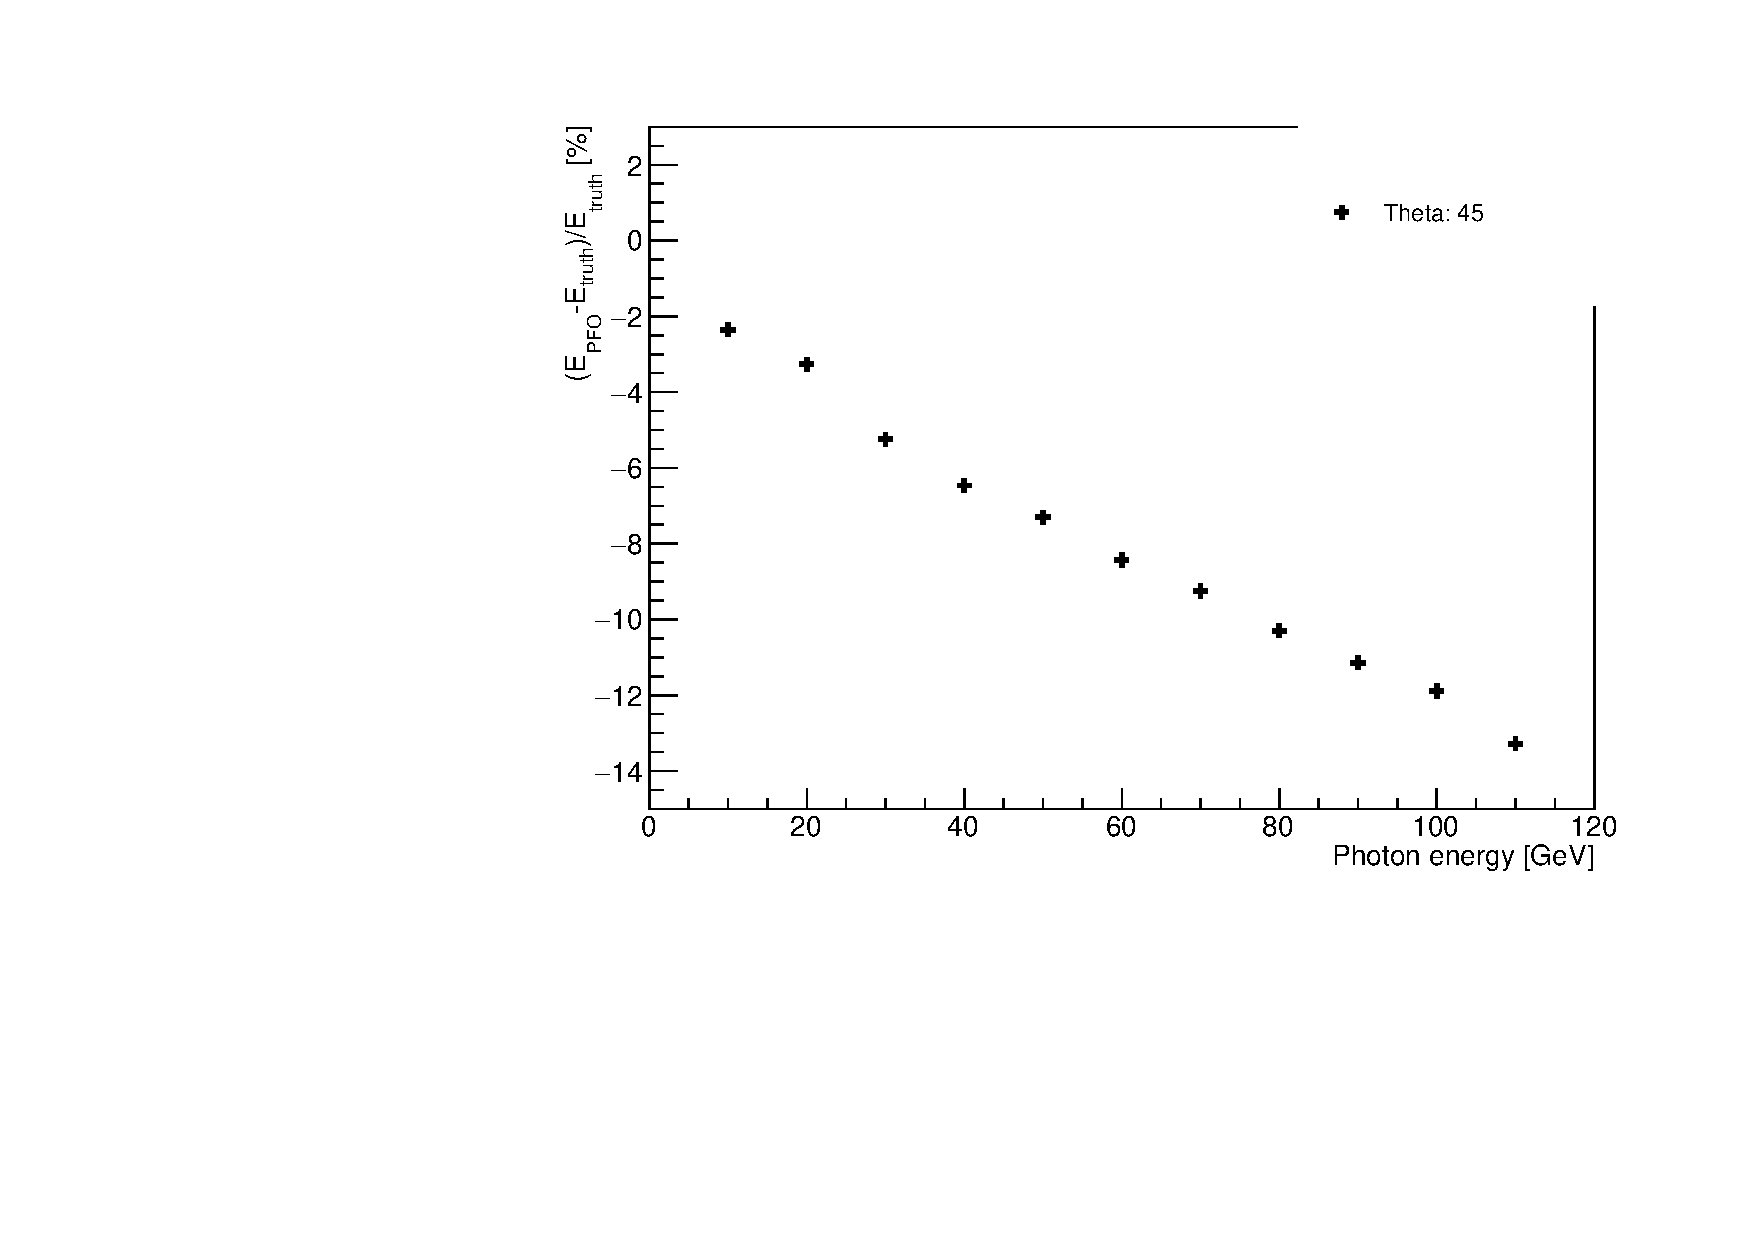
\includegraphics[width=6.5cm]{energyScaleBias_theta45_energy.pdf}};

 \node[inner sep=0pt] (tmp) at (\xRefPosOne+6,\yRefPosOne)
%     {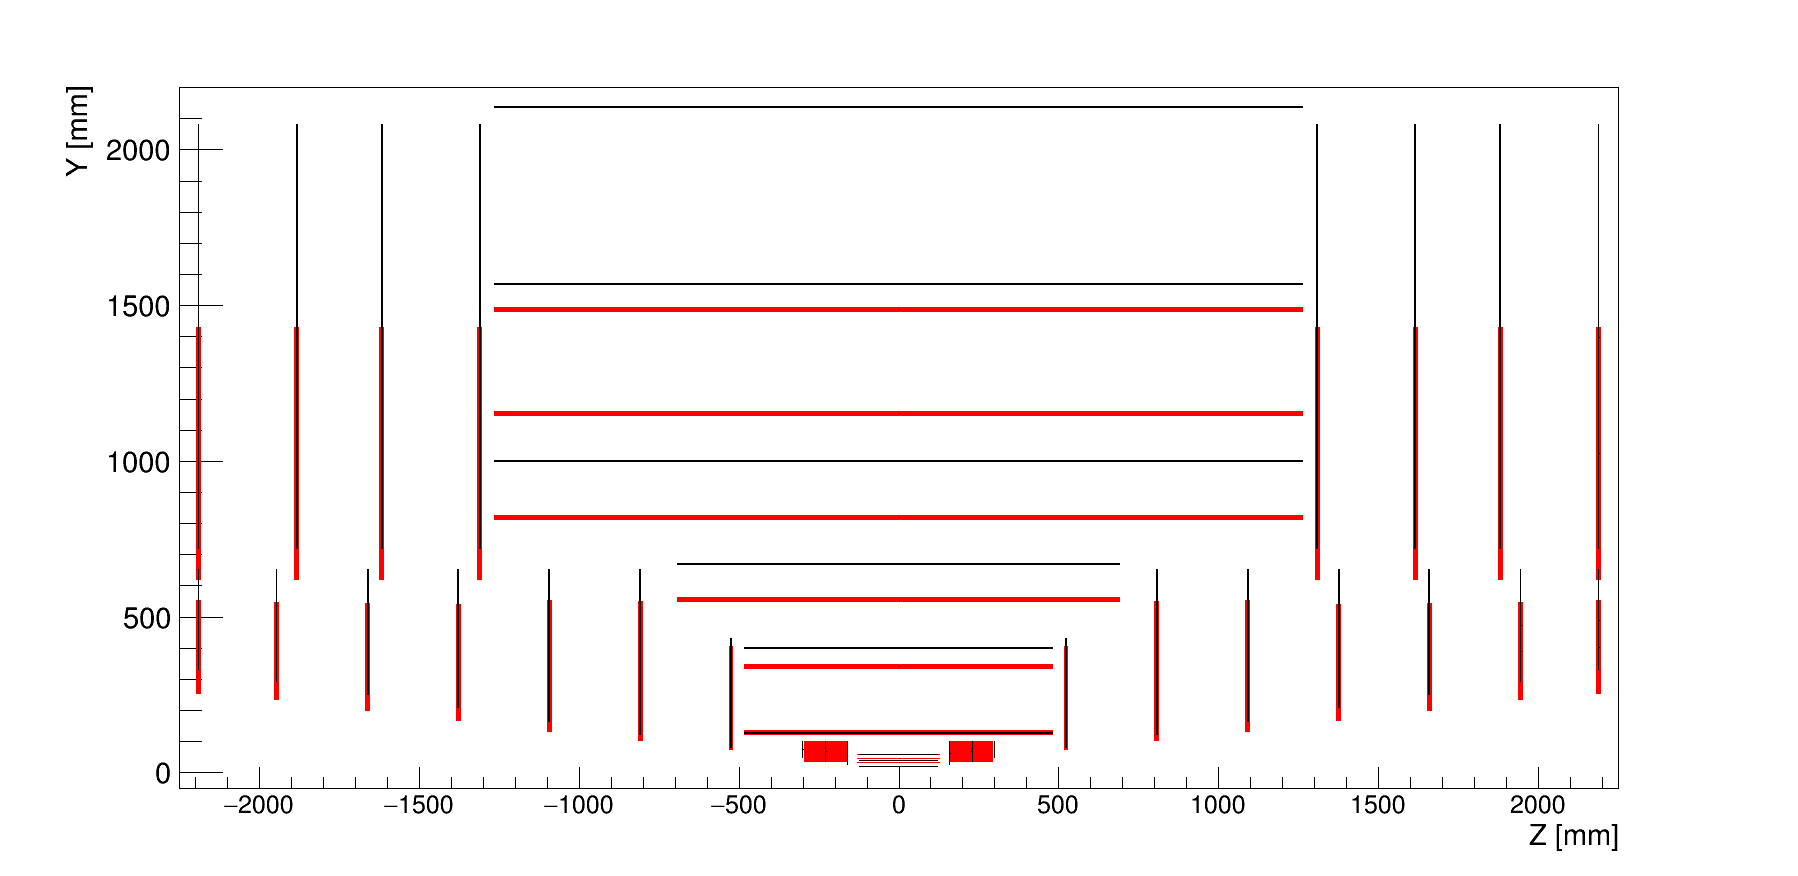
\includegraphics[width=12cm]{CLIC_vs_FCCee_trackingSystem.png}};
  {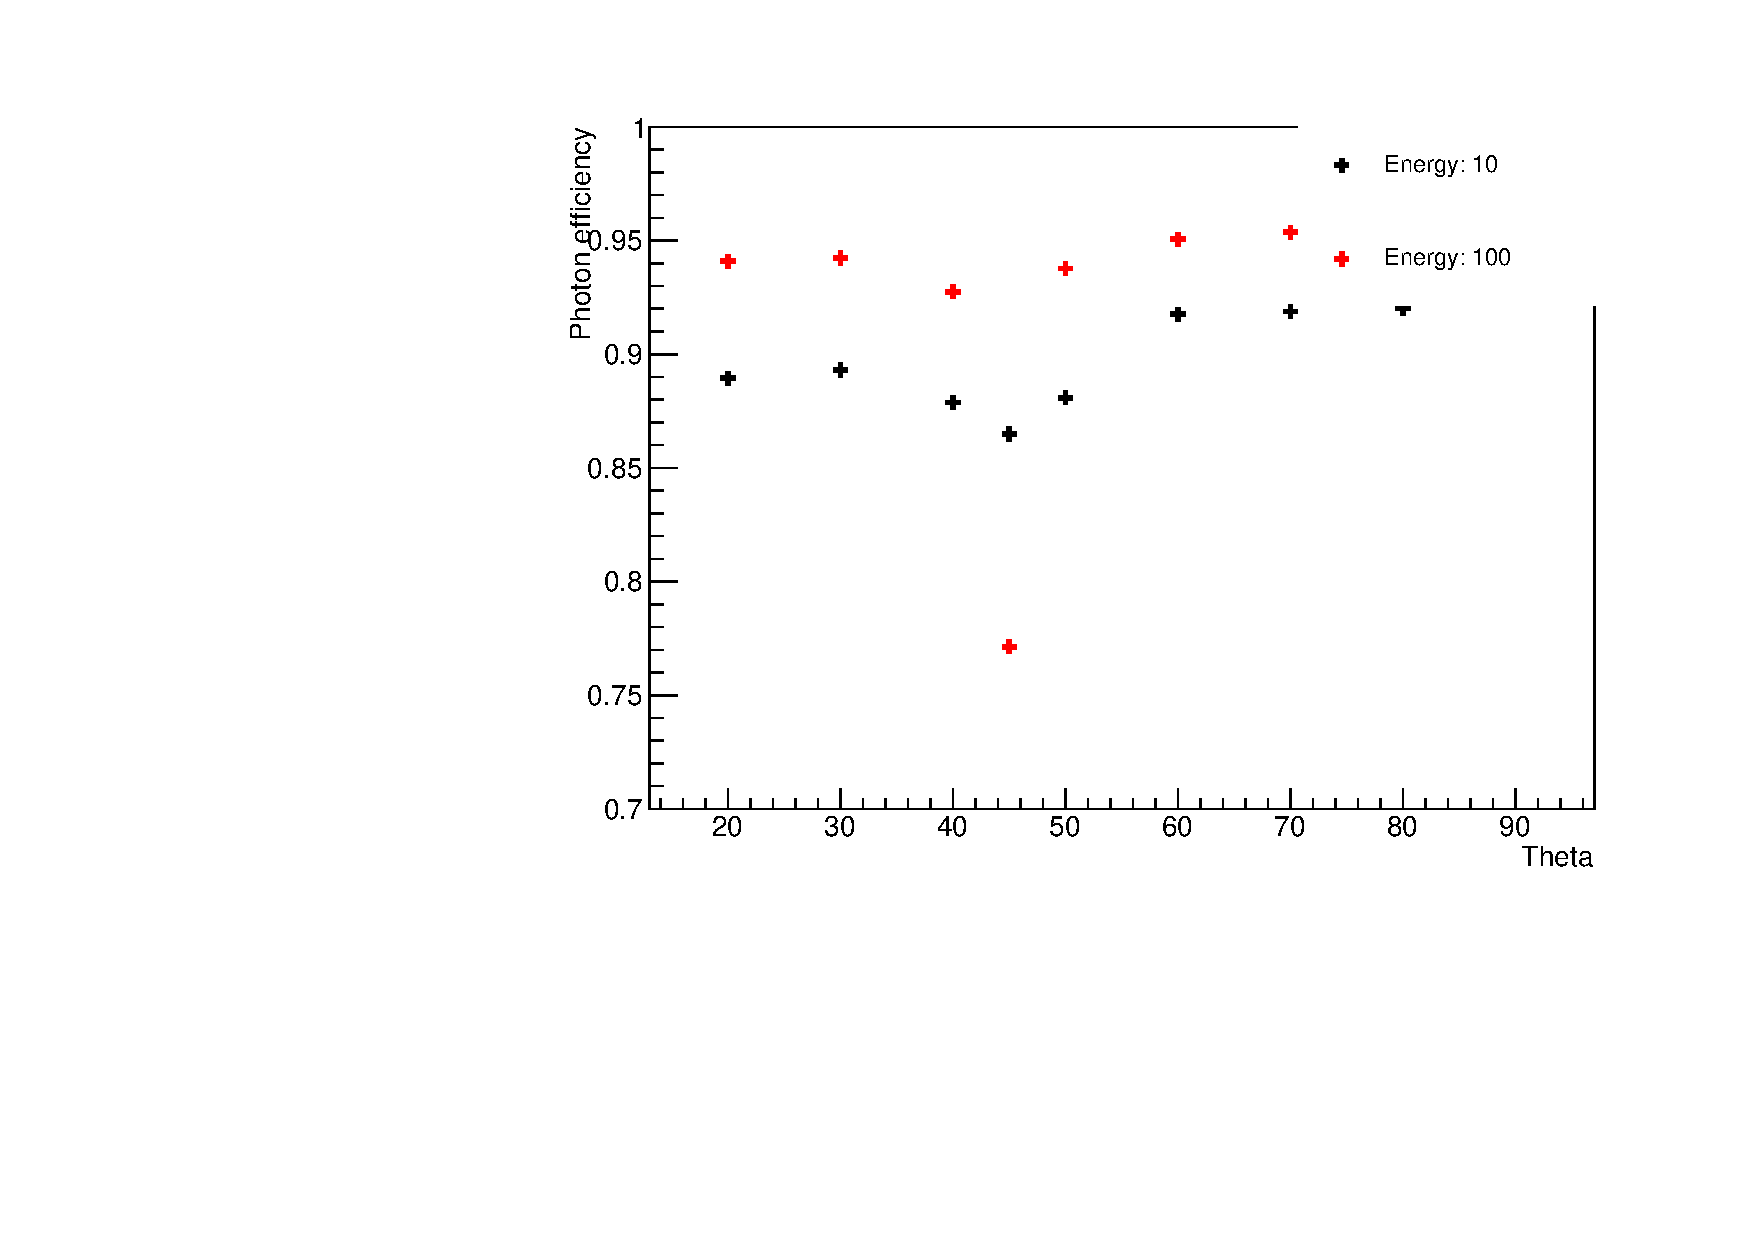
\includegraphics[width=6.5cm]{efficiency_theta.pdf}};

% 
% \node [Box] at (\xRefPosOne,\yRefPosOne+1.5) (box){%
% \myCenterBox{FCCee}
% };
% \node [Box] at (\xRefPosOne-2,\yRefPosOne+2) (box){%
% \myCenterBox{theta 80}
% };    
% 
% \node [Box] at (\xRefPosOne+5,\yRefPosOne+1.5) (box){%
% \myCenterBox{CLIC}
% };
% \node [Box] at (\xRefPosOne+5,\yRefPosOne+1) (box){%
% \myCenterBox{theta 90}
% };
% \node [Box] at (\xRefPosOne-2,\yRefPosOne-2.1) (box){%
% \myCenterBox{theta 80}
% };    
% 
\node [Box] at (\xRefPosOne+2.5,\yRefPosOne-3) (box){%
  \begin{minipage}{\textwidth}
    \begin{itemize}
      \item Some problems in the barrel-endcap transition region ($\approx$ 45$^{\circ}$)
      \item Need further investigation
    \end{itemize}
  \end{minipage}
};
%     
%% HELPER draw advanced helping grid with axises:
% \draw(-0.5,-4) to[grid with coordinates] (11.5,4);
\end{tikzpicture}

  
\end{frame}
%*****************************************************************************


\end{document}

